% \documentclass[review]{elsarticle}
\documentclass[]{elsarticle}

\usepackage{lineno,hyperref}
\modulolinenumbers[5]
\usepackage{xcolor}

\usepackage{amsmath,amsthm,amssymb}
\usepackage{enumitem}
% \usepackage[shortlabels]{enumerate}
\usepackage{tikz}
\usepackage{subfig}
\usepackage{graphicx}
\usepackage[toc,page]{appendix}

\usepackage{float}
   \restylefloat{figure}
   \restylefloat{table}

\usetikzlibrary{calc}
\usetikzlibrary{arrows.meta}
\usetikzlibrary{arrows}
\usetikzlibrary{shapes.geometric}
\tikzstyle{startstop} = [rectangle, rounded corners, minimum width=3cm, minimum height=1cm,text centered, draw=black, fill=red!20]
\tikzstyle{process} = [rectangle, minimum width=3cm, minimum height=1cm, text centered, draw=black, fill=orange!20]

\newcommand{\NN}{\mathbb{N}}
\newcommand{\ZZ}{\mathbb{Z}}
\newcommand{\QQ}{\mathbb{Q}}
\newcommand{\RR}{\mathbb{R}}
\newcommand{\CC}{\mathbb{C}}

\newcommand{\BB}{\mathcal{B}}
\newcommand{\CVect}{\CC\operatorname{-Vect}}
\newcommand{\Cantor}{\mathcal{C}}
\newcommand{\D}{\mathcal{D}}
\newcommand{\card}{\operatorname{card}}
\newcommand{\diam}{\operatorname{diam}}
\newcommand{\End}{\operatorname{End}}
\newcommand{\FF}{\mathcal{F}}
\newcommand{\GL}{\operatorname{GL}}
\newcommand{\Hom}{\operatorname{Hom}}
\newcommand{\id}{\operatorname{id}}
\newcommand{\Ind}{\operatorname{Ind}}
\newcommand{\interior}{\operatorname{int}}
\newcommand{\lcm}{\operatorname{lcm}}
\newcommand{\Lip}{\operatorname{Lip}}
\newcommand{\PGL}{\operatorname{PGL}}
\newcommand{\pic}{\vspace{30mm}}
\newcommand{\pset}{\mathcal{P}}
\newcommand{\Res}{\operatorname{Res}}
\newcommand{\Riem}{\mathcal{R}}
\newcommand{\RVect}{\RR\operatorname{-Vect}}
\newcommand{\Sch}{\mathcal{S}}
\newcommand{\SL}{\operatorname{SL}}
\newcommand{\supp}{\operatorname{supp}}

\newcommand{\Pcell}{P_{\text{cell}}}
\newcommand{\Pinf}{P_{\text{inf}}}
\newcommand{\Ppersist}{P_{\text{persist}}}
\newcommand{\Vdonor}{V_{\text{donor}}}
\newcommand{\Adonor}{A_{\text{donor}}}

\newcommand{\IFE}{\operatorname{IFE}}
\newcommand{\DFE}{\operatorname{DFE}}
\newcommand{\IE}{\operatorname{IE}}
\newcommand{\BRN}{\mathcal{R}_0}
\newcommand{\T}{CD4$^+$ T cells}

\newcommand{\SSR}{\operatorname{SSR}}

\renewcommand{\Re}{\operatorname{Re}}
\renewcommand{\Im}{\operatorname{Im}}

\newtheorem{theorem}{Theorem}[section]
\newtheorem{lemma}[theorem]{Lemma}
\newtheorem{corollary}[theorem]{Corollary}
\theoremstyle{definition}
\newtheorem{definition}[theorem]{Definition}
\newtheorem{remark}[theorem]{Remark}
\newtheorem{example}[theorem]{Example}
\newtheorem*{exer}{Exercise}



\usepackage{amsmath,amsthm,amssymb}
\usepackage{enumitem}


% Packages I can include or leave out as I see fit.
\usepackage{amsmath,mathtools}
\usepackage{amssymb}
\usepackage{amsthm}
\usepackage{graphicx}
\usepackage{caption}
\usepackage{float}
\usepackage{multirow}

\newcommand{\beq}{\begin{equation}}
\newcommand{\eeq}{\end{equation}}

\newcommand{\ba}{\begin{array}}
\newcommand{\ea}{\end{array}}

\newcommand{\bea}{\begin{eqnarray}}
\newcommand{\eea}{\end{eqnarray}}

\newcommand{\bc}{\begin{center}}
\newcommand{\ec}{\end{center}}

\newcommand{\ds}{\displaystyle}

\newcommand{\bi}{\begin{itemize}}
\newcommand{\ei}{\end{itemize}}

\newcommand{\bd}{\begin{description}}
\newcommand{\ed}{\end{description}}

\newcommand{\bp}{\begin{pmatrix}}
\newcommand{\ep}{\end{pmatrix}}

\newcommand{\beqq}{\begin{align*}}
\newcommand{\eeqq}{\end{align*}}





\journal{Mathematical Biosciences}

%%%%%%%%%%%%%%%%%%%%%%%
%% Elsevier bibliography styles
%%%%%%%%%%%%%%%%%%%%%%%
%% To change the style, put a % in front of the second line of the current style and
%% remove the % from the second line of the style you would like to use.
%%%%%%%%%%%%%%%%%%%%%%%

%% Numbered
%\bibliographystyle{model1-num-names}

%% Numbered without titles
%\bibliographystyle{model1a-num-names}

%% Harvard
%\bibliographystyle{model2-names.bst}\biboptions{authoryear}

%% Vancouver numbered
%\usepackage{numcompress}\bibliographystyle{model3-num-names}

%% Vancouver name/year
%\usepackage{numcompress}\bibliographystyle{model4-names}\biboptions{authoryear}

%% APA style
%\bibliographystyle{model5-names}\biboptions{authoryear}

%% AMA style
%\usepackage{numcompress}\bibliographystyle{model6-num-names}

%% `Elsevier LaTeX' style
\bibliographystyle{elsarticle-num}
%%%%%%%%%%%%%%%%%%%%%%%

\begin{document}

\begin{frontmatter}

\title{Modeling the effect of antibodies on the risk of HIV infection}


%% Group authors per affiliation:
% \author{Elsevier\fnref{myfootnote}}
% \fntext[myfootnote]{Since 1880.}

% \author{Angelica\fnref{myfootnote}}
% \fntext[myfootnote]{Since 1880.}
%% or include affiliations in footnotes:

\author[nav/ang]{Dr. Naveen K. Vaidya}
% \ead[url]{www.elsevier.com}
\author[carlos]{Carlos Villanueva Chavez}
\author[nav/ang]{Angelica Bloomquist \corref{mycorrespondingauthor}}
\cortext[mycorrespondingauthor]{Corresponding author}
\ead{abloomquist@sdsu.edu}
\author[aidan]{Aidan Backus}
\author[elyssa]{Elyssa Sliheet}
\author[J]{J Montgomery Maxwell}
\author[yuanming]{Yuanming Tang}

\address[nav/ang]{San Diego State University}
\address[carlos]{University of Oklahoma}
\address[aidan]{Brown University}
\address[elyssa]{Southwestern University}
\address[yuanming]{University of California, Berkeley}
\address[J]{Northwestern University}


\begin{abstract}

\textcolor{red}{EDIT THIS- probably will have a new abstract with the new organization of paper \\~\\
WANT TO CITE OUR OTHER PAPER TOO}

Over 36 million people currently live with the virus and approximately 1.8 million new infections are reported every year; the HIV epidemic continues to devastate worldwide. There is no cure for HIV, causing the lifelong persistence of the virus in infected individuals. The role of immune status of source partners should be considered while evaluating a risk of infection as suggested by experimental studies in which the immune status, primarily antibody levels, of source partners was found to have a significant impact on establishing infection in a new host. In this study, we developed two novel mathematical models of within-host HIV dynamics incorporating the effects of antibody levels of the source partners. These models allowed us to accurately estimate the probability of transmission, which appeared to be highly dependent upon the immune status of the source partners.
\end{abstract}

\begin{keyword}
Human immunodeficiency virus\sep mathematical models \sep risk of infection \sep antibodies
\end{keyword}

\end{frontmatter}

\linenumbers
\clearpage
\tableofcontents
\clearpage
\section{Introduction}

The HIV epidemic remains one of the most devastating problems worldwide. According to UNAIDS, in 2018 there were: 37.9 million people living with HIV/AIDS, 1.7 million new infections, 770 thousand deaths due to an AIDS-related illness. Even more surprisingly, only $79\%$ of all people living with HIV, knew their HIV status. That is, 8.1 million people did not know they were infected \cite{UNAIDS}. Given the persistence of new infections and the lack of prevention strategy, it is of paramount importance that we better understand HIV transmission dynamics. Therefore, in order to better control and prevent HIV endemics, it is crucial that we learn to quantify the risk of HIV infection.

Risk of HIV infection is defined as the probability that a susceptible, HIV-negative individual (recipient) is infected by HIV by means of contact of bodily fluids with an HIV-positive individual (donor). It has been established that the risk of infection is dependent on the mode of contact and the stage of infection of the host. Wawer et al. \cite{Uganda} has studied 235 HIV-discordant couples in Uganda and found that the rate of HIV transmission per coital act was highest (1 in 120) during acute-stage infection, but much lower (1 in 670) during chronic stage. Furthermore, Wawer is supported by a model in \cite{AntibodyIntroduction} which shows a connection between risk of infection, mode of contact and number of virus transferred. This model found that acute-stage donors have the highest probability of transmission and transfer by needlestick is generally riskier than sexual transmission, ceteris paribus.

Despite our continued advancements in the understanding of HIV, the effects of the donor's antibody profile on the risk of HIV infection have not been thoroughly explored. Research has illustrated that antibodies in the host are responsible for reducing risk of SIV infection in rhesus macaques \cite{bistableSwitch}, and Tomaras et al. \cite{Tomaras} has speculated that similar antibodies are responsible for binding to HIV viruses and reducing the risk of infection. Moreover, Vaidya et al. \cite{CHIDPatients} have found a significant correlation between the decay rate of virus infectivity and increase of plasma antibodies during HIV infection \cite{CHIDPatients}.

Mathematical models have proved fruitful for understanding the internal patterns of HIV infection. Since the early 1990's, models have shown that during the early stages of HIV infection, the viral load increases rapidly for the first weeks post-infection, reach a maximum, and then quickly decrease to a semi-steady state where it remains until treatment or AIDS begins \cite{Stafford2000}. However, it remains unknown whether the dramatic decline in viral load is principally the result of HIV-specific antibody responses or target cell limitation i.e., the exhaustion of new cells for HIV viruses to infect, as proposed by Phillips \cite{phillips1996reduction}.

In this paper we establish two viral-dynamics models that incorporate both viral load and HIV-specific antibody responses to quantify the risk of HIV infection for the first 500 days post infection. Approach 1 introduces antibodies into the basic viral dynamic model through a Hill function, while Approach 2 consists of an entirely new model centered around the effects of antibodies. Both of our models are parameterized in part, by using viral load and antibody data from six HIV infected individuals with an unusually early detection of HIV \cite{Tomaras}. The rest of the parameters were obtained through a data fitting process of the viral load and antibody data of the six patients. We then use the results from both models to examine how antibodies and the method of transmission affect the risk of infection. Our main reason for utilizing two different models is to compare results given the lack of research and to account for each model's shortcomings. In general, both models give almost identical results, however, we found Approach 1 enables more control over the effect of antibodies and is easier to model numerically, while Approach 2 is better suited for analytic results.

%%%%%%%%%%%%%%%%%%%%%%%%%%%%%%%%

\medskip

\section{Formulation of two approaches}

\subsection{Approach 1}
Model 1 in this study expands upon the standard HIV viral dynamics model. Following Mutua et al. \cite{pmid30931971}, we incorporate two effects of virus-specific antibodies: virus neutralization i.e. the reduction of virus infectivity with efficacy $\varepsilon_A$, and enhanced viral clearance as a result of an antibody binding to a cell-free virus with per-capita rate of $\mu A$. Throughout the paper, $A(t)$ represents the antibody profile of the host at time $t$. The efficacy of virus neutralization due to antibodies is modeled with the formula
$$\varepsilon_A = \frac{\eta A(t)}{1+\eta A(t)},$$
so that $\varepsilon_A=0$ in the absence of antibodies $(A = 0)$ and $\varepsilon_A \to 1$ as $A \to \infty$. Constants $\eta$ and $\mu$ are introduced in order to scale the net effect of viral neutralization, and viral clearance by antibodies on viral-dynamics. Note that $\eta = \mu = 0$ corresponds to the absence of antibodies.

As previously discussed, the behavior of virus-specific antibody data is low following infection, steadily increases to a maximum level, then sharply decreases to a near steady-state \cite{Stafford2000}. This prompts an immune response of HIV-specific antibodies which we model with the following Hill function.

$$A(t) = \frac{rt^n}{b^n+t^n},$$
where $r$ represents the maximum antibody level, $b$ represents the time post infection when half the antibody level is achieved, and $n$ is the Hill coefficient. Numerical values for $\mu,\eta, a,b, \text{and} n$ will be numerically estimated. Approach 1 is described by the following equations and schematic diagram:

	\begin{align}
	    \label{Approach I}
		\begin{cases}
			\dot{T} = \lambda-dT-(1-\varepsilon_A)kTV, &T(0) = T_0\\
			\dot{I} = (1-\varepsilon_A)kTV-\delta I, &I(0) = I_0\\
			\dot{V} = pI-cV-\mu A(t)V, &V(0) = V_0\\
		\end{cases}
	\end{align}

where $T,I,V$ represent the number of uninfected target CD4$^+$T cells, infected CD4$^+$T cells, and
virus, respectively. Target cells are produced at a rate $\lambda$, assumed to be independent of the state of infection, and die at rate $d$. Infected cells are produced with infection rate proportional to target cell and viral particles at rate $k$ and die at rate $\delta$. Viruses are produced by infected cells at rate $p$ per infected cell and are cleared at rate $c$.

\begin{figure}[H]
	\begin{center}
		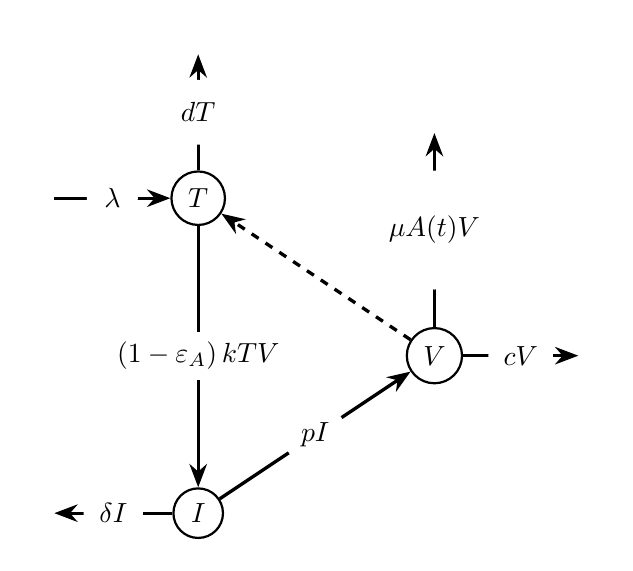
\begin{tikzpicture}
		\begin{scope}[every node/.style={circle,thick,draw}]
		\node[shape=circle,draw=black] (T) at (0,0) {$T$};
		\node[shape=circle,draw=black] (I) at (0,-4) {$I$};
		\node[shape=rectangle,draw=white] (kTV) at (0,-2) {$\left(1-\varepsilon_A\right)kTV$};
		\node[shape=circle,draw=black] (V) at (3,-2) {$V$};
		\end{scope}

		\begin{scope}[>={Stealth[black]},
		every node/.style={fill=white,circle},
		every edge/.style={draw=black,very thick}]
		\node (TA) at (-2, 0) {};
		\node (TB) at (0, 2) {};
		\node (IB) at (-2, -4) {};
		\node (VB) at (5, -2) {};
		\node (VC) at (3, 1) {};


		\path [->] (TA) edge node {$\lambda$} (T);
		\path [->] (T) edge node {$dT$} (TB);
		\path [-] (T) edge (kTV);
		\path [->] (kTV) edge (I);
		\path [->] (V) edge node {$cV$} (VB);
		\path [->] (I) edge node {$\delta I$} (IB);
		\path [->] (I) edge node {$pI$} (V);
		\path [->] (V) edge node {$\mu A(t)V$} (VC);
		\path [dashed, ->] (V) edge (T);
		\end{scope}
		\end{tikzpicture}
	\end{center}
	\caption{Approach 1 viral dynamics model}
\end{figure}


\subsection{Approach 2}

The main ideas behind this approach are to incorporate antibodies, $A$, into the model as a separate compartment and to divide the total viral load $V$ into two: infectious virus $V_I$ and noninfectious virus $V_N$.

Since some virus produced by the infected cells, $I$, can be non-infectious, we assume a fraction $\alpha \in [0,1]$ of newly produced virus becomes infectious and the remaining $(1-\alpha)\%$ are non-infectious. Following this assumption, we have infected cells producing infectious virus $V_I$ at a rate $\alpha p I$ and non-infectious virus $V_N$ being created at a rate of  $(1 - \alpha) p I$. Infectious virus and non infectious are both cleared by the body at a rate of $c$.

Since both infectious and non-infectious virus trigger production of antibodies, antibodies are produced at rate $\ell$ per virus and are cleared at a rate of $w$. We assume that antibodies neutralize infectious virus, i.e. converting $V_I$ into $V_N$, at rate $\sigma V_I A$.

Following the assumptions of this model, antibody neutralization of the virus reduces the infectivity of the virus (by converting infectious virus $V_I$ into non-infectious virus $V_N$) without diminishing total viral load $V = V_I + V_N$ in plasma. It is for this reason that we do not have a factor of $\left(1 - \varepsilon_A\right)$ on the term $kTV_I$, as seen in Approach 1. The reduced rate of infection in the previous approach $(1 - \varepsilon_A) k$ manifests here as a reduction of the infectivity of the virus, absorbed into the coefficient of the mass action term $\sigma$. This model does not have an enhanced clearance rate as approach 1 considers. (We note that this may be applied to model treatment, by assuming that a protease inhibitor reduces $\alpha$.)

A schematic diagram of Approach 2 is given in Figure \ref{Approach 2 diagram}. A summary of the parameters follows.

\begin{figure}[H]
\begin{center}
	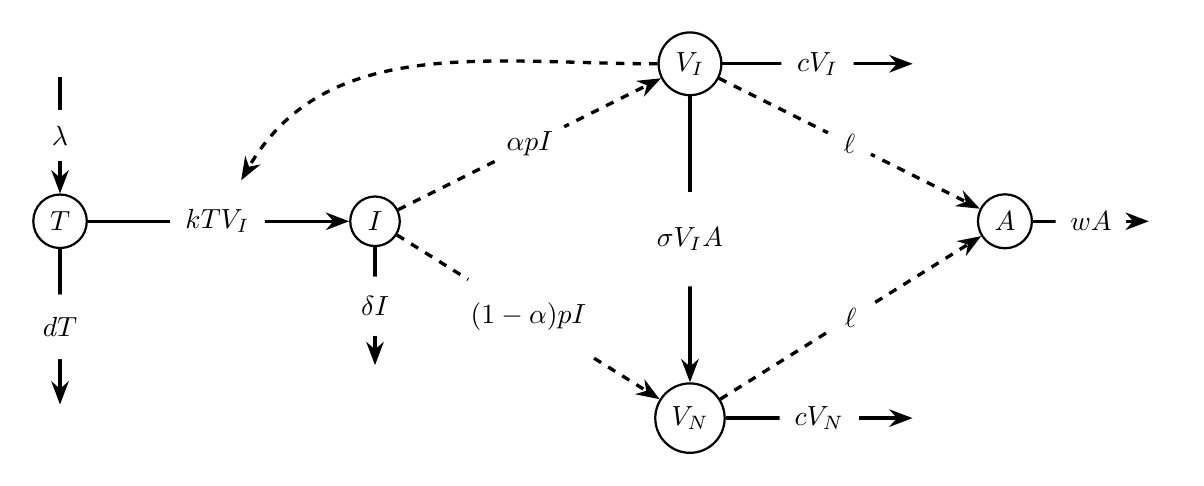
\begin{tikzpicture}
	\begin{scope}[every node/.style={circle,thick,draw}]
	\node[shape=circle,draw=black] (T) at (-4,3) {$T$};
	\node[shape=circle,draw=black] (I) at (0,3) {$I$};
	\node[shape=circle,draw=black] (VI) at (4,5) {$V_I$};
	\node[shape=circle,draw=black] (VN) at (4,.5) {$V_N$};
	\node[shape=circle,draw=black] (A) at (8,3) {$A$};
	\node[draw=none, fill=none] (kTV) at (-2,3){$kTV_I$};

	\end{scope}

	\begin{scope}[>={Stealth[black]},
	every node/.style={fill=white,circle},
	every edge/.style={draw=black,very thick}]
	\node (TN) at (-4, 5) {};
	\node (TD) at (-4, .5) {};
	\node (ID) at (0,1) {};
	\node (VID) at (7, 5) {};
	\node (VND) at (7, .5) {};
	\node (AD) at (10, 3) {};
	\path [dashed, ->] (I) edge node {$\alpha pI$} (VI);
	\path [dashed, ->] (I) edge node {$(1-\alpha) pI$} (VN);
	\path [->] (VI) edge node {${\sigma} V_I A$} (VN);
	\path [->] (TN) edge node {$\lambda$} (T);
	\path [->] (T) edge node {$dT$} (TD);
	\path [->] (I) edge node {$\delta I$} (ID);
	\path [->] (VI) edge node {$cV_I$} (VID);
	\path [->] (VN) edge node {$cV_N$} (VND);
	\path [->] (A) edge node {$wA$} (AD);
	\path [dashed, ->] (VI) edge node {${\ell}$} (A);
	\path [dashed, ->] (VN) edge node {${\ell}$} (A);
	\path [-] (T) edge (kTV);
	\path [->] (kTV) edge (I);
	\draw [dashed, ->,black,very thick] (VI) to [out=180, in = 60] (kTV);


	\end{scope}
	\end{tikzpicture}
\end{center}
	\caption{Approach 2 viral dynamics model}
	\label{Approach II diagram}
\end{figure}

\begin{align}
\label{Approach II}
\begin{cases}
\dot{T} = \lambda-dT-kTV_I,\> T(0) = T_0 \\
\dot{I} = kTV_I-\delta I,\>I(0) = I_0 \\
\dot{V_I} = \alpha pI-cV_I-\sigma V_I A ,\>V_I(0) = V_{I0} \\
\dot{V_N} = (1-\alpha)pI+\sigma V_I A -cV_N ,\>V_N(0) = V_{N0}\\
\dot{A} = \ell(V_I+V_N)-wA,\>A(0) = A_0\\
\end{cases}
\end{align}

\subsection{Initial Conditions}
We adopt the convention similar to that in \cite{sachsenberg1998turnover}, that the count of CD4$^+$T cells is multiplied by $1\%$. It follows that the initial condition on target cells ,$T_0$, is taken to be $10^4$ per ml. We assume this is the start of infection, thus there are no infected cells yet, so $I_0 = 0$ and $\dot T(0)= 0$; therefore $\lambda = dT_0$. The initial virus concentration is often unknown, but here we take $V_{I0} = 1/300$ initial virus RNA copies per ml. Antibody production is triggered by the creation of virus, therefore $A_0 = 0$. We will assume in Approach 2 that $V_{N0} = 0$.


\section{Formulation of Risk}


We define the risk of infection, $\Pinf$, as the probability of a successful establishment of HIV infection in a susceptible individual. For a susceptible individual (recipient) to be infected by HIV through a single contact with an HIV-infected individual (donor), the following conditions have to be satisfied:

\begin{enumerate}
    \item the virus has to reach the target cells (transmission)
    \item at least one target cell has to be infected by the virus (infection initiation)
    \item the infected target cell has to establish a persistent infection (persistence)
\end{enumerate}

The process, and the probability of a successful infection through a single contact, is depicted in Figure \ref{diagram}.

\begin{figure}[H]
\tikzstyle{line} = [draw, -latex']
\tikzstyle{startstop} = [rectangle, rounded corners, minimum width=8cm, minimum height=1cm,text centered, draw=black, fill=red!20]
\tikzstyle{process} = [rectangle, minimum width=12cm, minimum height=1cm, text centered, draw=black, fill=orange!20]
\begin{center}
	\begin{tikzpicture}[node distance = 2cm, auto]
	%place nodes
    	\node(host) [startstop] {HIV-positive donor};
	    \node(virus) [process, below of = host] {HIV-positive bodily fluid containing HIV and antibodies};
    	\node(cross) [process, below of =virus] {Virus and antibodies cross mucus membranes of the recipient};
    	\node(Pcell) [process, below of =cross] {CD$4^+$ T cell of recipient infected};
    	\node(recipient) [startstop, below of =Pcell] {Infection persists in susceptible recipient};
    	\path [line] (host) --node[text width =4cm]{$m_1$} (virus);
    	\path [line] (virus) --node[text width =4cm]{$m_2$} (cross);
    	\path [line] (cross) --node[text width =4cm]{$\Pcell$} (Pcell) ;
    	\path [line] (Pcell) --node[text width =4cm]{$\Ppersist$} (recipient);
	\end{tikzpicture}
	\caption{Schematic diagram leading to a successful infection in a recipient}
	\label{diagram}
\end{center}
\end{figure}

\subsection{Transmission}
Depending on the mode of transmission, we assume some small fraction, $m= m_1m_2$, of the virus and antibodies in the bloodstream of the donor actually survive the transmission process, where $m_1$ is the scaling factor relating concentrations in the donor blood and released bodily fluid (e.g. semen), and $m_2$ is the proportion of released virus that enters the recipient bloodstream.

We let $a$ denote the age of infection of the donor, i.e. the time since the onset of infection in the donor. In this notation, $m\Vdonor(a)$ virions and $m\Adonor(a)$ free antibodies are transmitted and reach the target cells of the recipient. This transmission term will be incorporated for both approaches.


\subsection{Infection Initiation}

Suppose that virions infect target cells at a rate $\rho$ per virus, and let
\begin{equation}
    \label{average infected number of target cells}
    \gamma(t) = \rho \int_0^t V(s) ~ds
\end{equation}
be the expected number of infections in target cells in the new host before time $t$. We assume that new infections follow an inhomogeneous Poisson process; then the probability of $x$ target cells being infected is $\gamma^x e^{-\gamma} (x!)^{-1}$.

In particular, the probability that no cells are infected before time $t$ is $e^{-\gamma(t)}$ \cite{AntibodyIntroduction}. It follows that the probability that at least one cell is infected before time $t$ is $\left(1 - e^{-\gamma(t)}\right)$. Moreover, the probability that at least one cell is ultimately infected is
\begin{equation}
    \label{eventual infection probability}
    \Pcell = \lim_{t \to \infty} \left(1 - e^{-\gamma(t)}\right).
\end{equation}

Per our model as well as empirical evidence, the host will not produce a significant number of antibodies for the first few weeks, so we make the approximating assumption that all free antibodies are those transmitted by the donor, and not produced by the recipient. Therefore, $\dot A + wA = 0$, and in particular $A(t) = \Adonor(a) e^{-wt}$. We also assume $I = 0$ because no cells have been infected yet.

\subsection{Persistence}

HIV is known to persist as a chronic illness for several years in its host before the onset of AIDS. Both of these models will have two equilibria, an infectious free equilibrium $(\IFE)$ and an infectious equilibrium $(\IE)$. $\IE$ is defined to be the steady state of the system, which can be interpreted as its behavior in chronic phase if the effects of AIDS are ignored.

Given a single cell is successfully infected, we now formulate the probability, $P_\text{persist}$, that the initiated infection establishes a persistent infection. For this, we again assume the inhomogeneous Poisson process, with the basic reproduction number, $\BRN$, serving as a new Poisson parameter representing the expected number of secondary infections from a single infected cell, if the infected cell is introduced into an otherwise healthy population \cite{DefiningBRN}.

We denote by $T_0$ the initial condition on target cells, $T_0 = \lambda/d$. Let us define the \emph{biologically feasible region} $\overline \BB$ to be the state space satisfying the constraints $T \in [0, \lambda/d]$, $I \geq 0$, $V_I \geq 0$, $V_N \geq 0$ and $A \geq 0$. (Note that for Approach I, we take $V_I = V$, $V_N = 0$, and $A = 0$.) We demand that $T \leq \lambda/d$ since $\dot T \leq \lambda - dT$, so if $T(0) = \lambda/d$ is taken as an initial condition, it follows that $T \leq T_0$. Define the \emph{infectious vector} $X = (I, V_I)$, and define the \emph{infectious region} $\BB$ to be the interior $\{(T, I, V_I, V_N, A) \in \: T < T_0 \text{ or } |X| > 0\}$.


However, the corresponding system for Approach 1 is underdetermined, so we can only show
\begin{align*}
    T^* &= \frac{\lambda}{d} - \frac{\delta}{dp^2}(c^2 - \delta^2M^2)I\\
    pI^* &= (c - \delta M)V
\end{align*}
in that case.

In numerical experiments, it became clear that as the time $t \to \infty$, the state approached $\IE$ whenever $\BRN > 1$. On the other hand, if $\BRN^{II} < 1$, $V_I^* < 0$, which lies outside of $\overline \BB$ and is absurd, so there is no endemic equilibrium.

It is quite difficult to prove that $\IE$ is stable when $\BRN > 1$, because the model is highly nonlinear there. But recall that an infection is said to be \emph{uniformly persistent} if for each solution curve $(T, X, V_N, A)$ such that the infectious vector $X$ satisfies $X(t) > 0$ for some $t > 0$, $\liminf_{t \to \infty} |X(t)| > 0$. That is, an infection is uniformly persistent if it cannot resolve itself in finite time (say, without introducing treatment). Provided that $\BRN > 1$, the infection is uniformly persistent.

In contrast to the above, the infection will resolve itself whenever $\BRN < 1$. The local stability of deterministic compartmental models of the form given was proven by Van den Driessche and Watmough \cite{van2002reproduction}, but we will be able to prove \emph{global} stability.

\begin{theorem}[global stability of $\IFE$]
\label{ife_theorem}
    Suppose that $\BRN < 1$. Then the $\IFE$ is both locally and globally asymptotically stable for both Approaches.
\begin{proof}
See \ref{global1} and \ref{global2}.
\end{proof}
\end{theorem}

\begin{theorem}[uniform persistence]
\label{IE}
    If $\BRN < 1$, the infection will not persist. Conversely, if $\BRN > 1$, the model is uniformly persistent for both Approaches and an infectious equilibrium exists.
\begin{proof}
    The case $\BRN < 1$ follows from Theorem \ref{ife_theorem}. For the converse, see Appendix \ref{pers}.
\end{proof}
\end{theorem}

Previously we have treated the qualitative dynamics of the deterministic models given at the beginning of this paper. But in considering the probability of transmission, we are not justified in using the deterministic models: in this case, the infectious vector $X$ is close to $0$, and so it is plausible that the infection would resolve itself even if $\BRN > 1$ due to effects not considered by the deterministic model. However, it is known that the conditional probability of persistence given that a single cell has already been infected is $\Ppersist = 1 - \exp \BRN$ \cite{pPersist}. We let $\Pinf$ denote the probability of infection and $\Pcell$ denote the probability that a single cell is infected, so that
$$\Pinf = \Pcell \Ppersist.$$

%%%%%%%%%%%%%%%%%%%%%%%%%%%%%
%%%%%%%%%%%%%%%%%%%%%%%%%%%%%
%%%%%%%%%%%%%%%%%%%%%%%%%%%%%
%%%%%%%%%%%%%%%%%%%%%%%%%%%%

\section{Risk of infection}

Let $\rho$ denote the rate at which cells are infected per virus and per unit time, and let $\nu$ denote the ratio of infectious viruses to total viruses transferred. (In Approach 1, $\nu = 1$, and $V_I = V$.)

If we ignore the $T$ and $I$ terms in the model, and assume that no new antibodies are being created, then
$$-\frac{\dot V_I}{V_I} = c + \sigma A,$$
and integrating both sides, we have
\begin{align*}
    \ln\left(\frac{V_I(0)}{V_I(t)}\right) &= ct + \sigma \int_0^t A(s) ~ds\\
    &= ct + m\sigma \Adonor(a) \int_0^t e^{-ws}~ds \\
    &= ct + \frac{m\sigma}{w} \Adonor(a) (1 - e^{-wt}).
\end{align*}
Exponentiating both sides and taking reciprocals,
\begin{equation}
\label{viral load after infection}
    \frac{V_I(t)}{V_I(0)} = e^{-ct}\exp\left(-\frac{m\sigma}{w}\Adonor(a)(1-e^{-wt}\right).
\end{equation}
We note that (\ref{viral load after infection}) is valid provided that the virus has not infected any cells in its new host and that the host has not started to produce new antibodies -- this is why we were able to discard terms in the derivation of (\ref{viral load after infection}).

Plugging (\ref{viral load after infection}) into (\ref{average infected number of target cells}) and (\ref{eventual infection probability}), we conclude that for Approach 2,
\begin{equation}
    \Pcell^I(a) = 1 - \exp\bigg\{-(1 - \varepsilon_{m\Adonor(a)}) kT_0m\Vdonor(a)
   \int_0^{\infty} \exp\left[-cs - \frac{m\mu \Adonor(a)}{w}(1 - e^{-ws})\right] ~ds\bigg\}.
    \label{pcell1}
\end{equation}
Similarly, for Approach 2,
\begin{equation}
    \Pcell^{II}(a)= 1 - \exp\bigg\{-kT_0mV_{I\text{ donor}}(a)\int_0^{\infty}\exp\left[-cs - \frac{m\sigma \Adonor(a)}{w}(1 - e^{-ws})\right] ~ds\bigg\}.
    \label{pcell2}
\end{equation}

In order to use the next-generation matrix method to compute $\BRN$, we need to compute the Jacobian matrix of the system linearized about the infectious free equilibrium, $\IFE = (\frac{\lambda}{d}, 0, 0)$ at time $t = 0$, taking only the infectious compartments. For Approach 1, we have
$$J = \begin{bmatrix}-\delta & \frac{k\lambda}{d}\\p &-c
\end{bmatrix}.$$
Splitting up $J$ such that $J=F-V$, we have
$$F = \begin{bmatrix}0& \frac{k\lambda}{d}\\ p&0\end{bmatrix}, \hspace{5mm}
V =  \begin{bmatrix} \delta & 0\\ 0&c\end{bmatrix}.$$

The basic reproduction number is found by taking the spectral radius of $FV^{-1}$. We find
$$\BRN^I = \frac{kp\lambda}{cd\delta}.$$
Plugging this in as a Poisson parameter,
\begin{equation}
    P_\text{persist}^I = 1-\exp\left(\frac{kp\lambda}{cd\delta}\right).
    \label{ppersist1}
    \end{equation}

Now let $J$ be the Jacobian matrix of the Approach 2 system, again linearized about $\IFE = (\lambda/d, 0, 0, 0, 0)$ and with only infectious compartments, so that
$$J = \begin{bmatrix}
    -\delta & \frac{k\lambda}{d}& 0\\
    \alpha p & -c & 0\\
    (1-\alpha)p & 0 & -c\end{bmatrix}.$$
By a similar computation to as in Approach I, with $V = \operatorname{diag}(\delta, c, c)$,
$$FV^{-1} = \begin{bmatrix}
    0 & \frac{k\lambda}{dc} & 0\\
    \frac{\alpha p}{\delta} & 0 & 0\\
    \frac{(1-\alpha)p}{\delta} & 0 & 0
\end{bmatrix},$$
so
$$\BRN^{II} = \frac{kp\alpha\lambda}{cd\delta}.$$

Therefore
\begin{equation}
    P_\text{persist}^{II} = 1 - \exp\left(\frac{kp\alpha\lambda}{cd\delta}\right).
    \label{ppersist2}
\end{equation}


%%%%%%%%%%%%%%%%%%%%%%%%%%%%%
%%%%%%%%%%%%%%%%%%%%%%%%%%%%%
%%%%%%%%%%%%%%%%%%%%%%%%%%%%%
%%%%%%%%%%%%%%%%%%%%%%%%%%%%







%%%%%%%%%%%%%%%%%%%%%%%%%%%%%%%%%%%%%%%%%%%%%%%%%%%%%%%%%%%%%%%%%%%%%%%%%%%%%%%%%%%%%%%%%%%%%%%%%%%%%%%%%%%%%%%

\section{Computation of Risk of Infection}

\subsection{Data Fitting and Parameter Estimation}

Data fitting was used for all the parameters that were not already biologically known such as $\lambda, p$ and $c$, where $\lambda = dT_0$ \cite{stafford2000modeling}, $p = 5000$ \cite{vaidya2018correlation} and $c = 23$ \cite{wei2003antibody}

\subsubsection{Approach 1}
For each patient's antibody function $A(t)$, the parameters $r$, $b$, and $n$ were obtained by fitting the curve to antibody data (recorded in optical density) using MATLAB's ``Curve Fitting" tool. Afterwards, we incorporated each patient's antibody function $A(t)$ into Approach 1 and numerically solved the system of ODEs to estimate $\mu, \eta,k, \delta, $ and $d$. The predicted $\text{log}_{10}$ viral load values were fitted to each patient's viral load data $(v_\ell)$ using the fmincon solver in MATLAB to minimize the sum of square residuals (SSR).

For Approach 1, we defined the SSR to be
$$\SSR = \sum (\text{log}_{10}(V-v_{\ell}))^2,$$

Figures \ref{app1ant} and \ref{app2viral} show the resulting curve fitting for each patient's antibody and viral load respectively.

% The median values in the antibody function were estimated to be $a = 2.476, b = 23.115,$ and $n = 20.96 $. That is, the median of the maximum antibody load is 2.476 O.D. where half of the load is achieved after 23.115 days. Overall, we found the median values to be consistent with each patient's individual values with the exception of $\sigma$ whose values were evenly distributed from a low of 1.0372 ml ng$^{-1}$ day$^{-1}$ to a high of 9.0483 ml ng$^{-1}$ day$^{-1}$. We concede this is most likely due to the limited amount of patient data available. However, there is undoubtedly a correlation between parameters. For example, patient CHID79 yielded the lowest $\mu$, $\eta$, $a$, and $n$ values while patient CHID32 yielded the highest $\mu$ and $\eta$ values as well as the lowest $b$ value.

Table \ref{app1values} summarizes the data-fitted parameters for each patient.


\begin{table}[H]
\footnotesize
\centering
\begin{tabular}{|l|l|l|l|l|l|l|l|l|}
\hline
Patient   & r & b & n   & $\mu$ & $\eta$ & $k$ & $\delta$ &  $d$  \\
\hline
CHID46 &  3.647 & 20.22 & 128  &2.1464 & 0.3683 & $7.92\cdot 10^{-7}$ & 0.2322 &  0.0191  \\\hline
CHID77 & 2.082 & 24.14 & 42.4 & 4.3371 & 0.3329 & $7.43\cdot10^{-7}$ & 0.2449 & 0.0133  \\\hline
CHID79 & 1.917 & 22.54 & 2.454& 1.0372 & $2.93\cdot10^{-4}$ & $9.00\cdot10^{-7}$ & 0.3483 & 0.0187 3 \\\hline
CHID32& 2.484 & 20.72 & 16.85 & 9.0483 & 0.6663 & $7.28\cdot10^{-7}$ & 0.3175 & 0.0229  \\\hline
CHID40 & 3.122 & 23.69 & 17.43& 5.1887 & 0.3683 & $7.26\cdot10^{7}$ & 0.2337& 0.0151  \\\hline
CHID08 & 2.468 & 25.75 & 24.49 & 7.2609 & 0.6121 & $7.35\cdot10^{-7}$ & 0.2073 & 0.0119  \\\hline
median &2.476 & 23.115 & 20.96& 4.76   & 0.368  & $7.39\cdot10^{-7}$ & 0.2393  & 0.0169  \\\hline
\end{tabular}
\caption{Approach 1 parameters}
\label{app1values}
\end{table}

\begin{figure}[H]
	\centering
		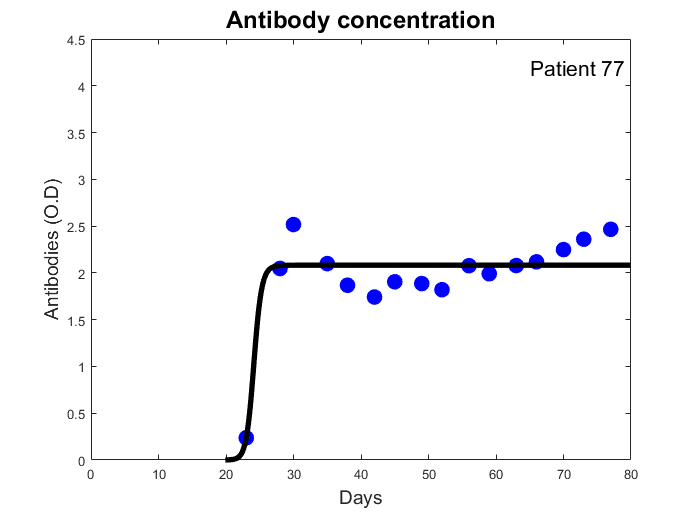
\includegraphics[width=.32\linewidth]{data_fit_app1/CHID77a.png}
		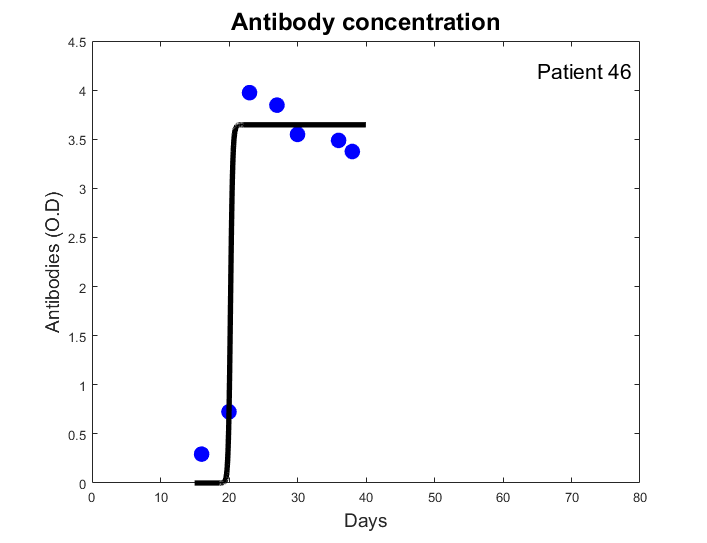
\includegraphics[width=.32\linewidth]{data_fit_app1/CHID46a.png}
		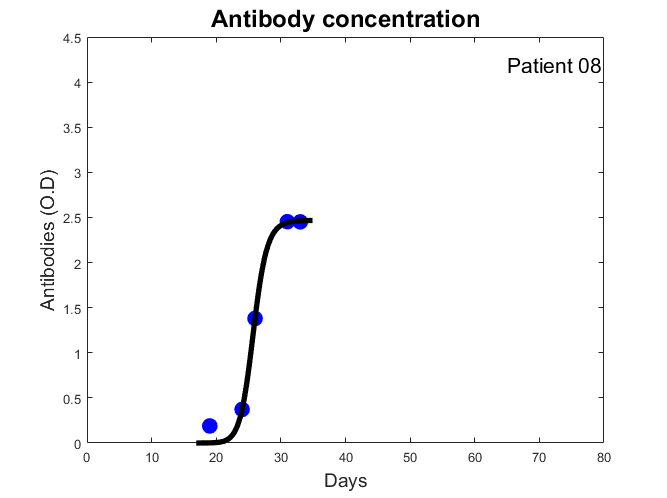
\includegraphics[width=.32\linewidth]{data_fit_app1/CHID08a.png}
		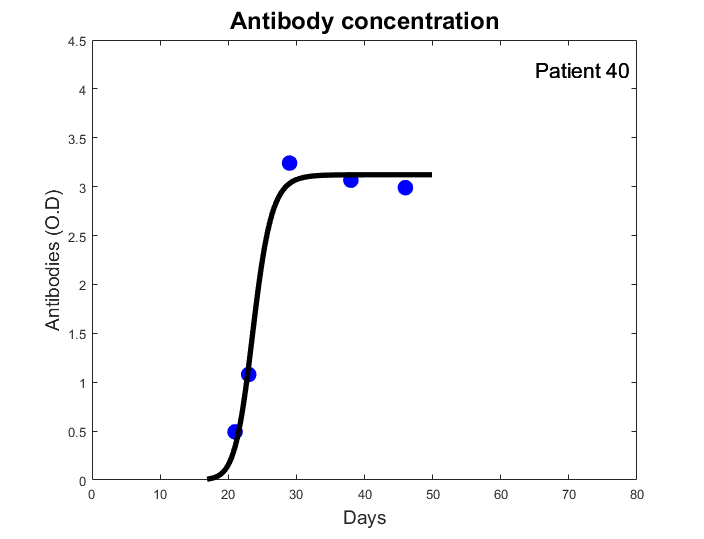
\includegraphics[width=.32\linewidth]{data_fit_app1/CHID40a.png}
		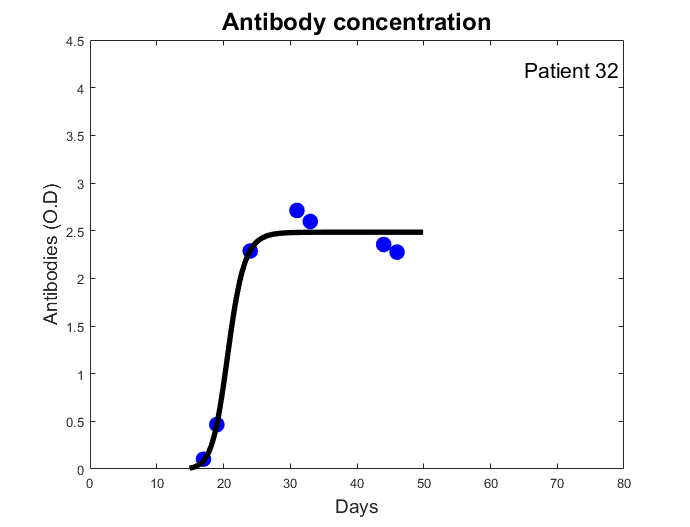
\includegraphics[width=.32\linewidth]{data_fit_app1/CHID32a.png}
		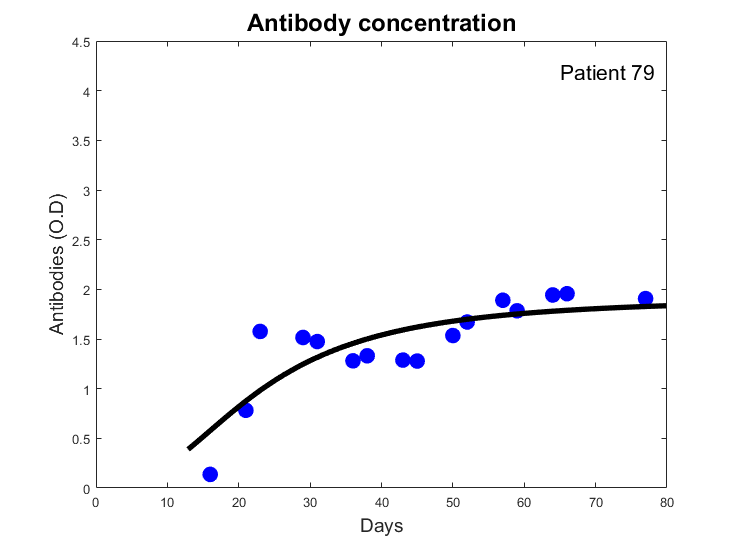
\includegraphics[width=.32\linewidth]{data_fit_app1/CHID79a.png}
	\caption{Approach 1 antibody curve fitting
	\label{app1ant}}
\end{figure}

\begin{figure}[H]
	\centering
		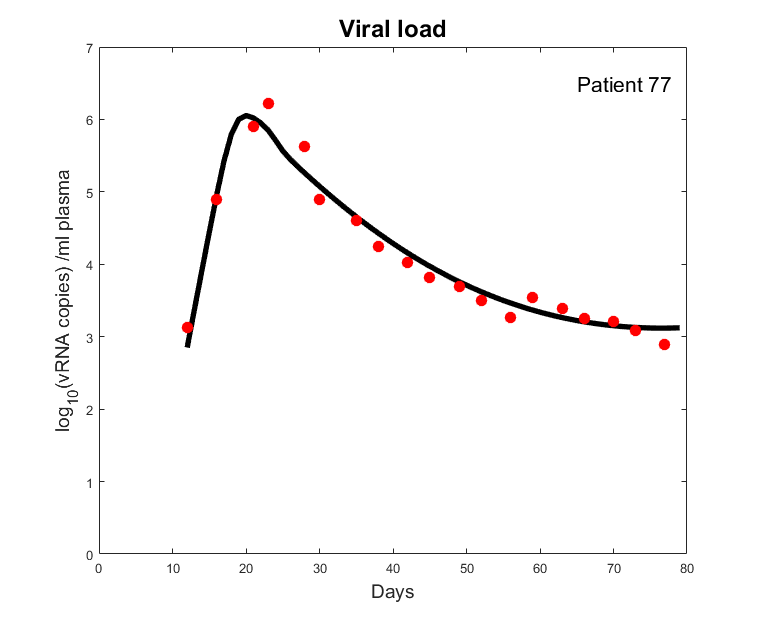
\includegraphics[width=.32\linewidth]{data_fit_app1/CHID77v.png}
		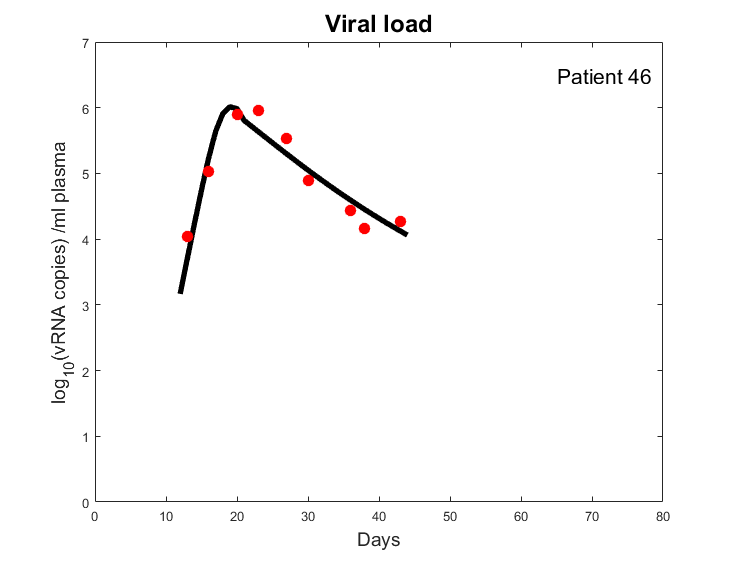
\includegraphics[width=.32\linewidth]{data_fit_app1/CHID46v.png}
		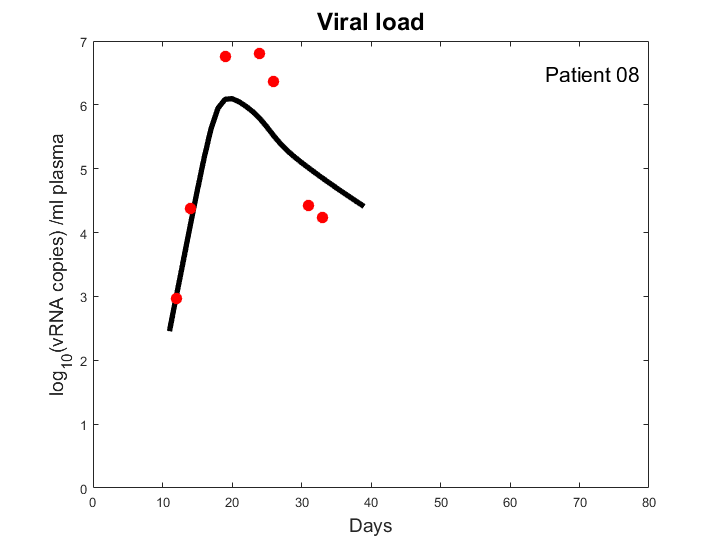
\includegraphics[width=.32\linewidth]{data_fit_app1/CHID08v.png}
		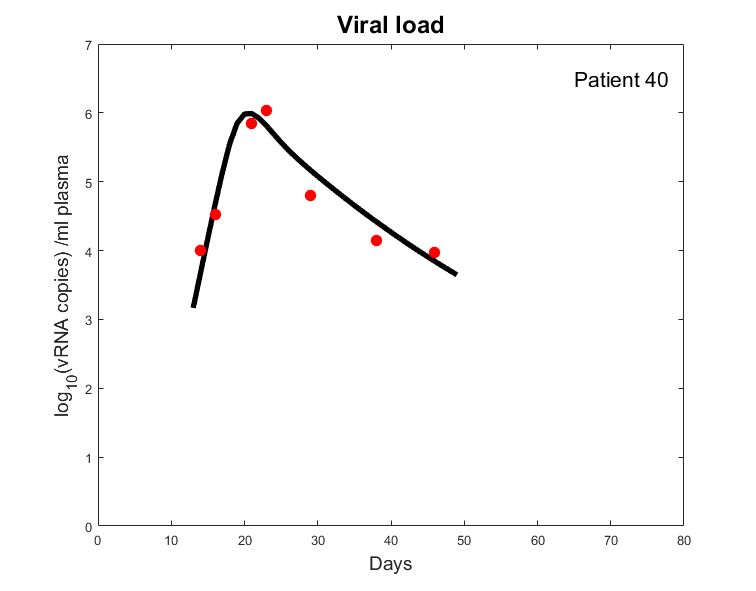
\includegraphics[width=.32\linewidth]{data_fit_app1/CHID40v.png}
		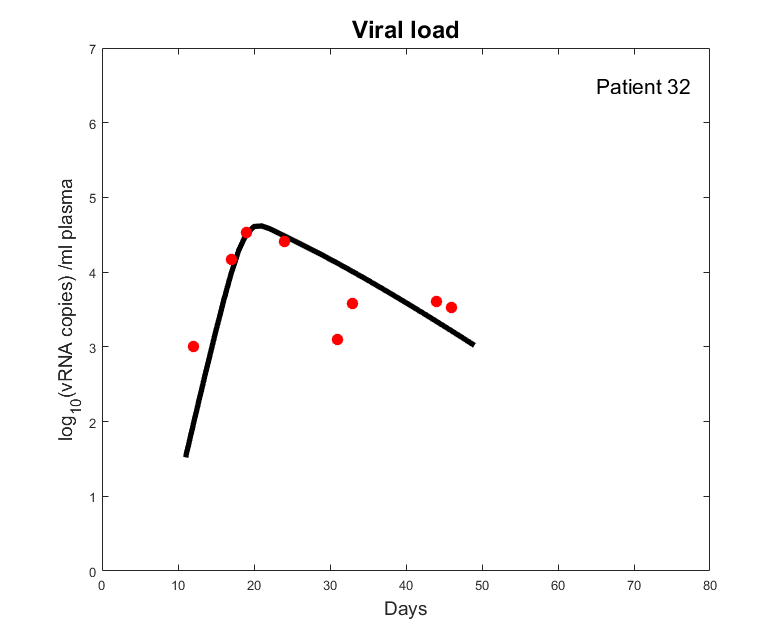
\includegraphics[width=.32\linewidth]{data_fit_app1/CHID32v.png}
		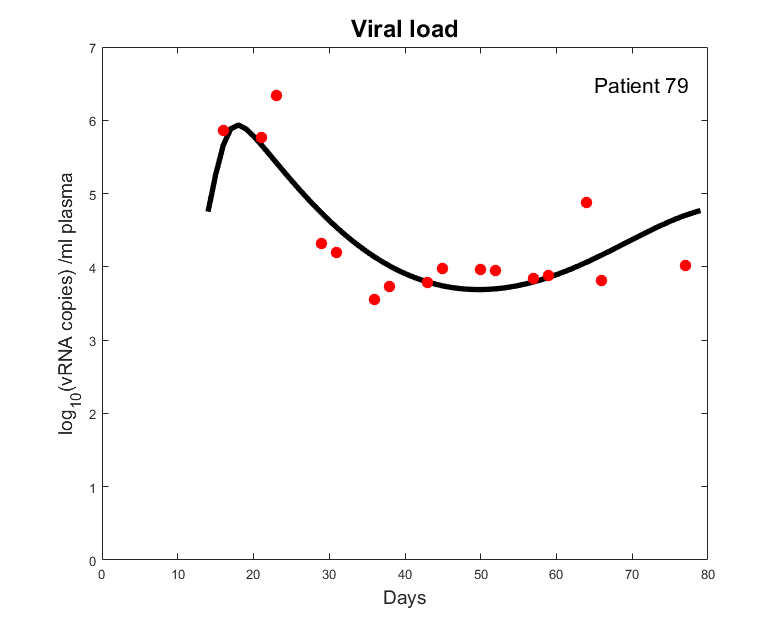
\includegraphics[width=.32\linewidth]{data_fit_app1/CHID79v.png}
	\caption{Approach 1 viral load curve fitting \label{app1viral}}
\end{figure}

\subsubsection{Approach 2}
For parameter estimation in Approach 2, both viral load and antibody concentration of the patients were fitted against the model. We data fitted to estimate the following parameters: $\ell, w, \sigma, k, \delta$ and $d$.

We define
$$\SSR = \sum \left((\log_{10} (V_I +V_N)-v_\ell)+(A-a_\ell) \right)^2$$
where $v_\ell$ and $a_\ell$ are the patient's viral and antibody data respectively at various time points. Minimizing the SSR gave us the following parameter estimates.



\begin{centering}
\begin{table}[H]
% \scriptsize
\begin{tabular}{|c|c|c|c|c|c|c|c|}
\hline
Patient & $\ell$ & $w$ & $\sigma$ & $k$ & $\delta $ & $d$ \\ \hline
CHID46 &$6.95 \cdot 10^{-7}$&0.0326	&	12.775&	 $8.23\cdot 10^{-7}$&  0.27&	0.01	\\ \hline
CHID77 & $2.44\cdot 10^{-7}$	&$1.45\cdot 10^{-7}$&	13.805&	$8.13\cdot 10^{-7}$&	0.272&		0.0107\\ \hline
CHID79 & $2.49 \cdot 10^{-7}$ &	$7.3 \cdot 10^{-10}$ &	0.0017&	$9.49 \cdot 10^{-7}$&	0.362&		0.0129	\\
\hline
CHID32 &$3.43 \cdot 10^{-6}$	&0.0404	&13.056	&$9.908 \cdot 10^{-7}$&	0.523	&	0.03	 \\ \hline
CHID40 & $7.059  \cdot 10^{-7}$&	0.0083	&13.127&	$8.718 \cdot 10^{-7}$&	0.286&		0.027 \\ \hline
CHID08 &$1.774 \cdot 10^{-7}$ &$3.679 \cdot 10^{-7}$&	13.702&	$7.918 \cdot 10^{-7}$ &	0.195	&0.01	\\ \hline
median&$4.72 \cdot 10^{-7}$	&$4.15  \cdot 10^{-3}$&	13.092&	$8.47  \cdot 10^{-7}$&	0.279&	.0118	\\ \hline
average &$9.16  \cdot 10^{-7}$&	0.01355&	11.078&	$8.73  \cdot 10^{-7}$&	0.318&		0.0168	\\ \hline
\end{tabular}
\caption{Approach 2 parameters}
\label{table:ta}
\end{table}
\end{centering}

\begin{figure}[H]
\begin{centering}
		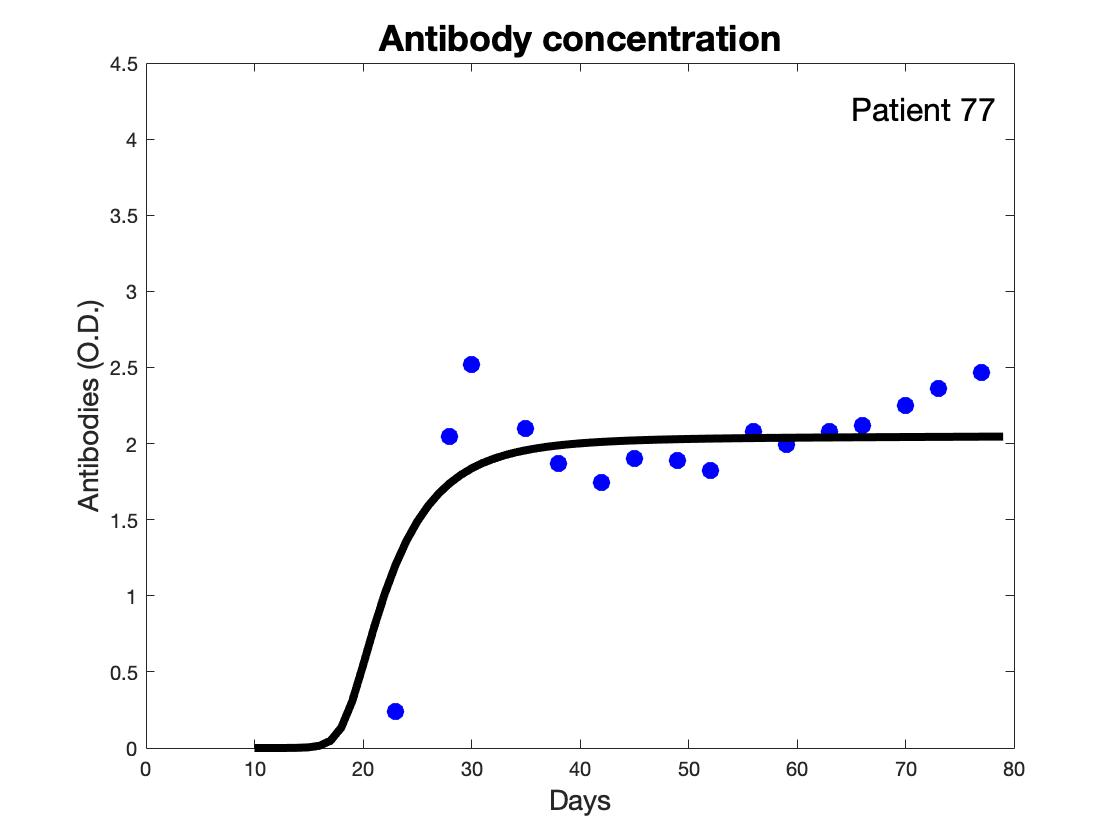
\includegraphics[width=.325\linewidth]{data_fit_app2/77a.jpg}
		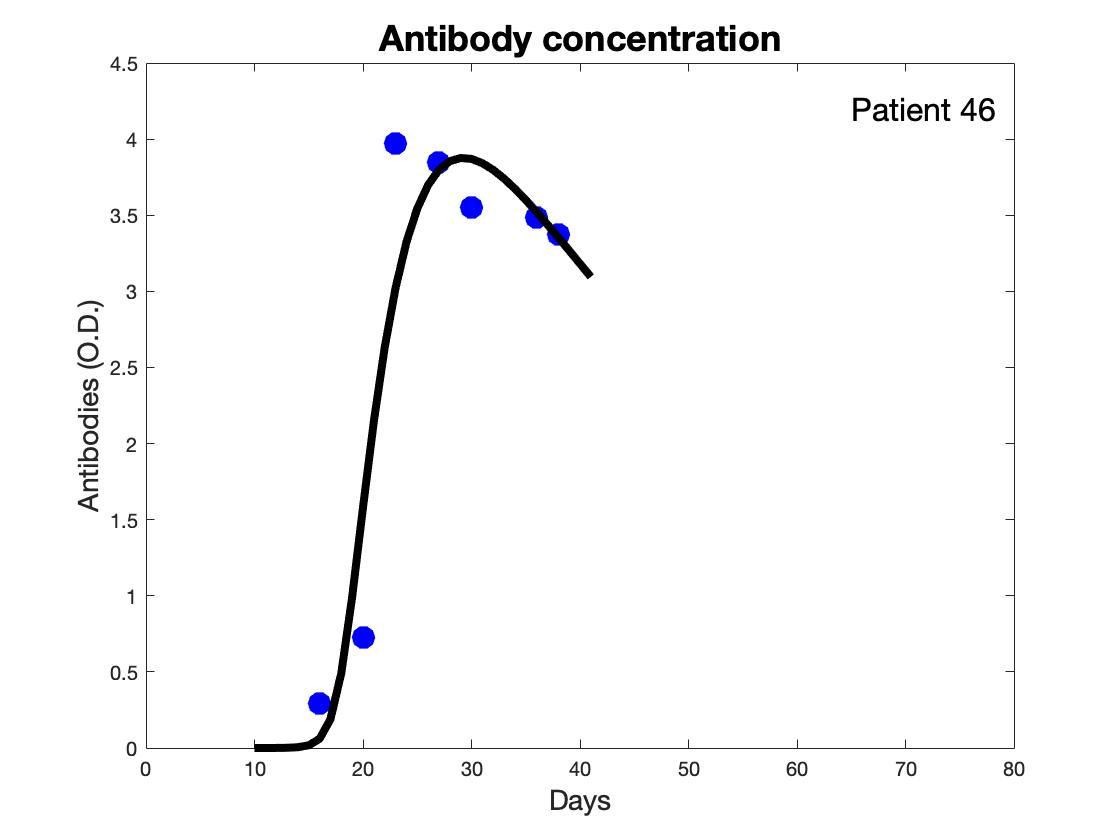
\includegraphics[width=.325\linewidth]{data_fit_app2/46a.jpg}
		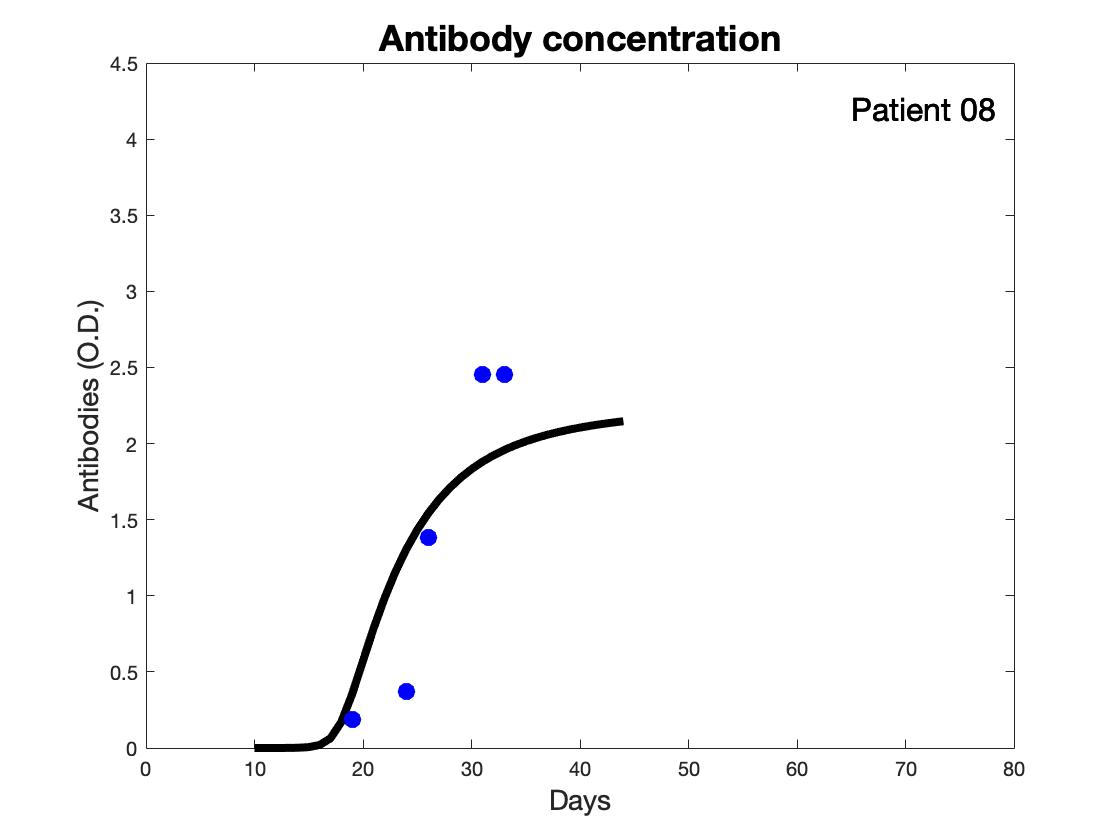
\includegraphics[width=.325\linewidth]{data_fit_app2/8a.jpg}
		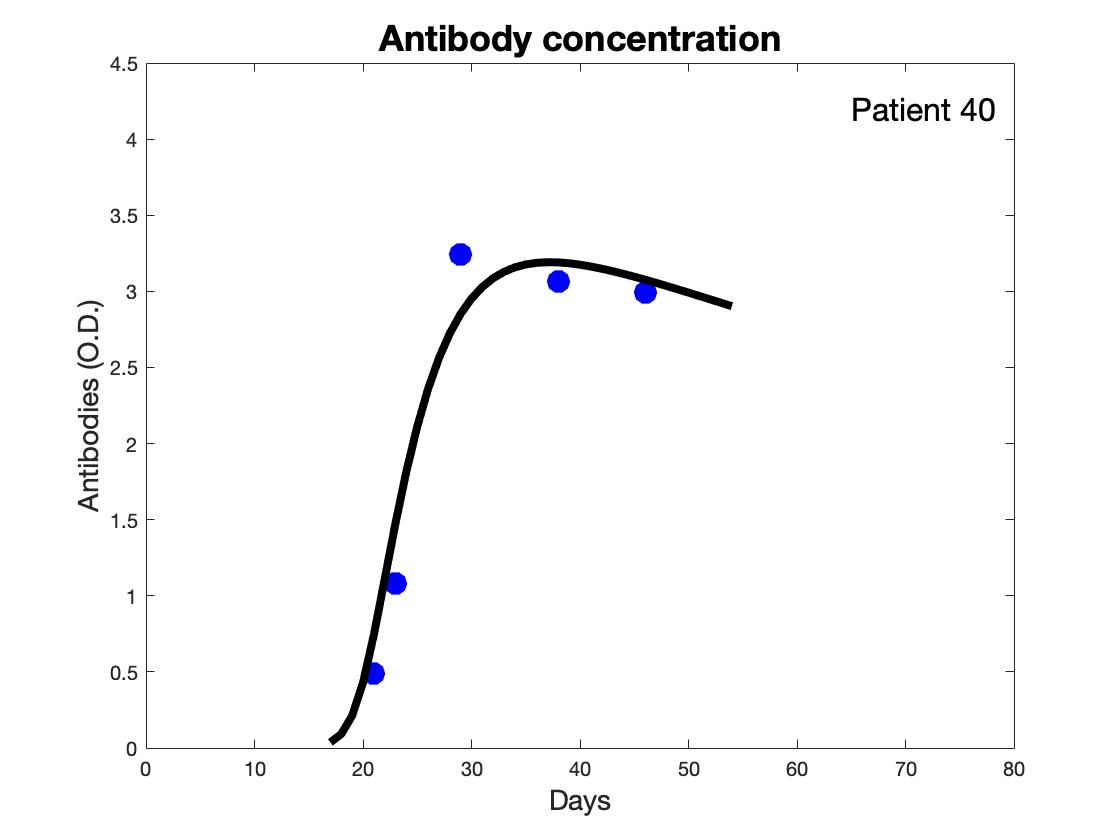
\includegraphics[width=.325\linewidth]{data_fit_app2/40a.jpg}
		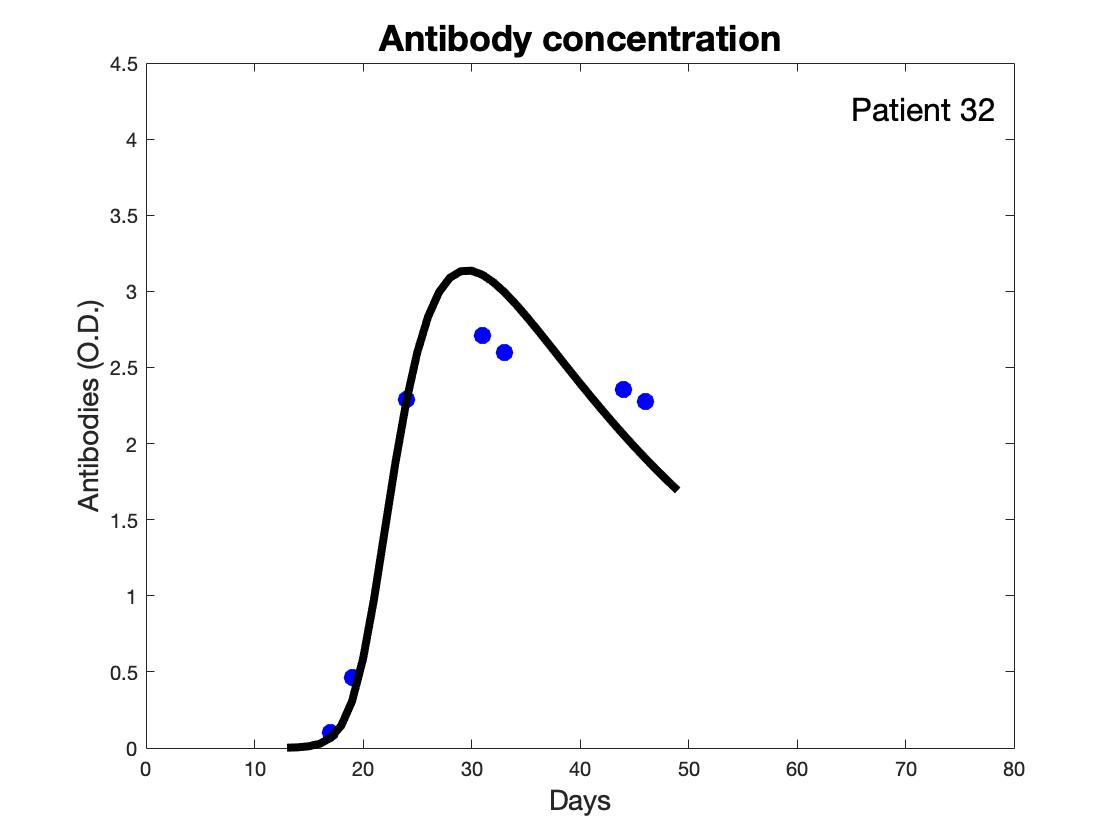
\includegraphics[width=.325\linewidth]{data_fit_app2/32a.jpg}
		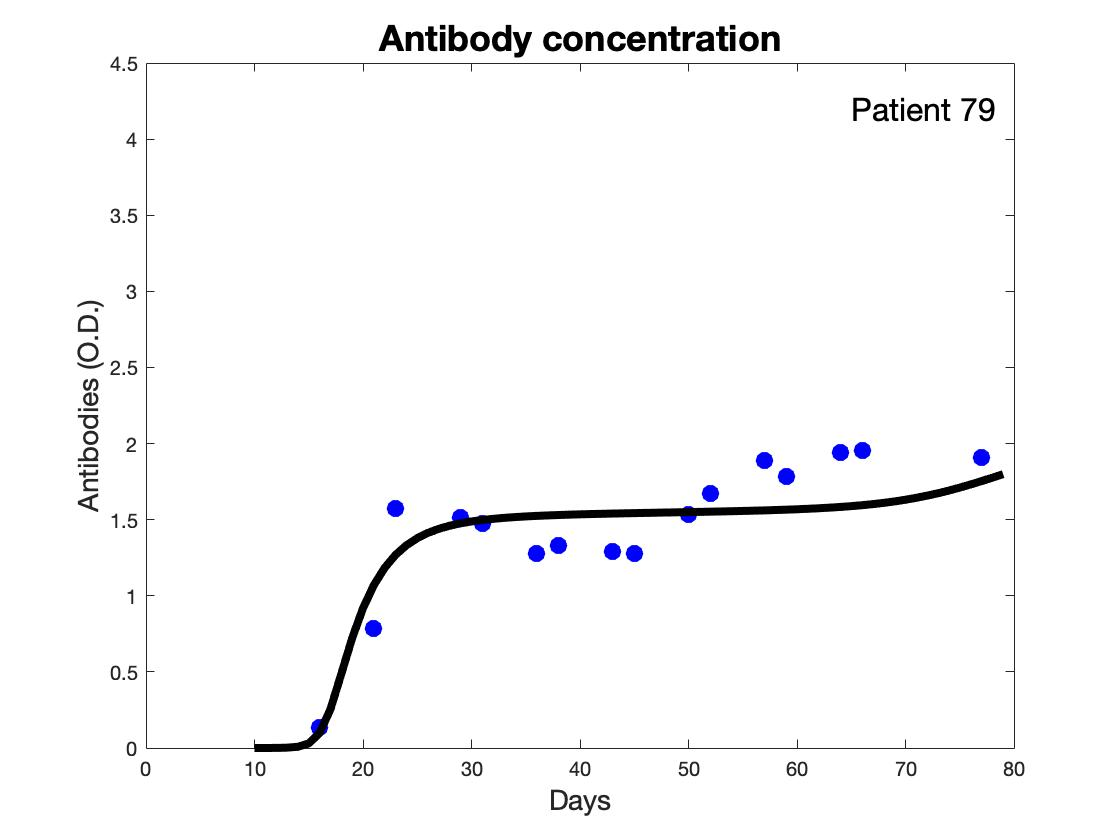
\includegraphics[width=.325\linewidth]{data_fit_app2/79a.jpg}
	\caption{Approach 2 antibody curve fitting}
	\label{app2ant}
	\end{centering}
\end{figure}

\begin{figure}[H]
	\centering
		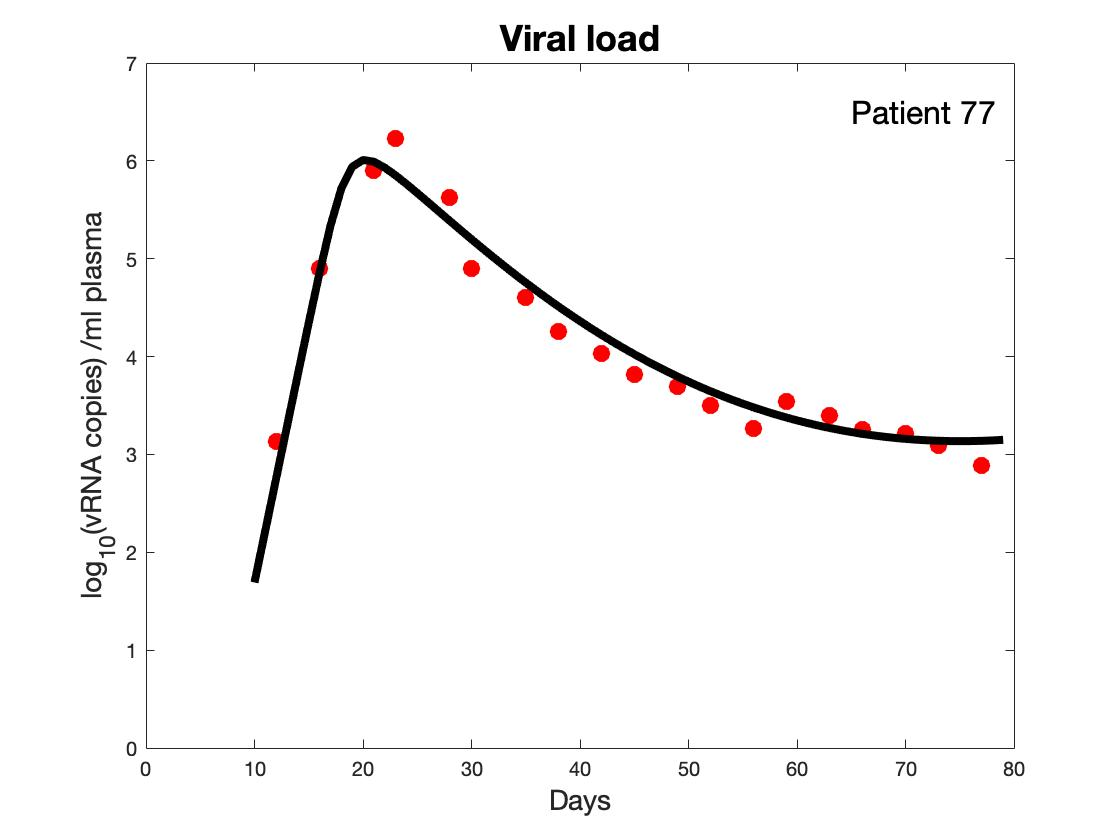
\includegraphics[width=.32\linewidth]{data_fit_app2/77v.jpg}
		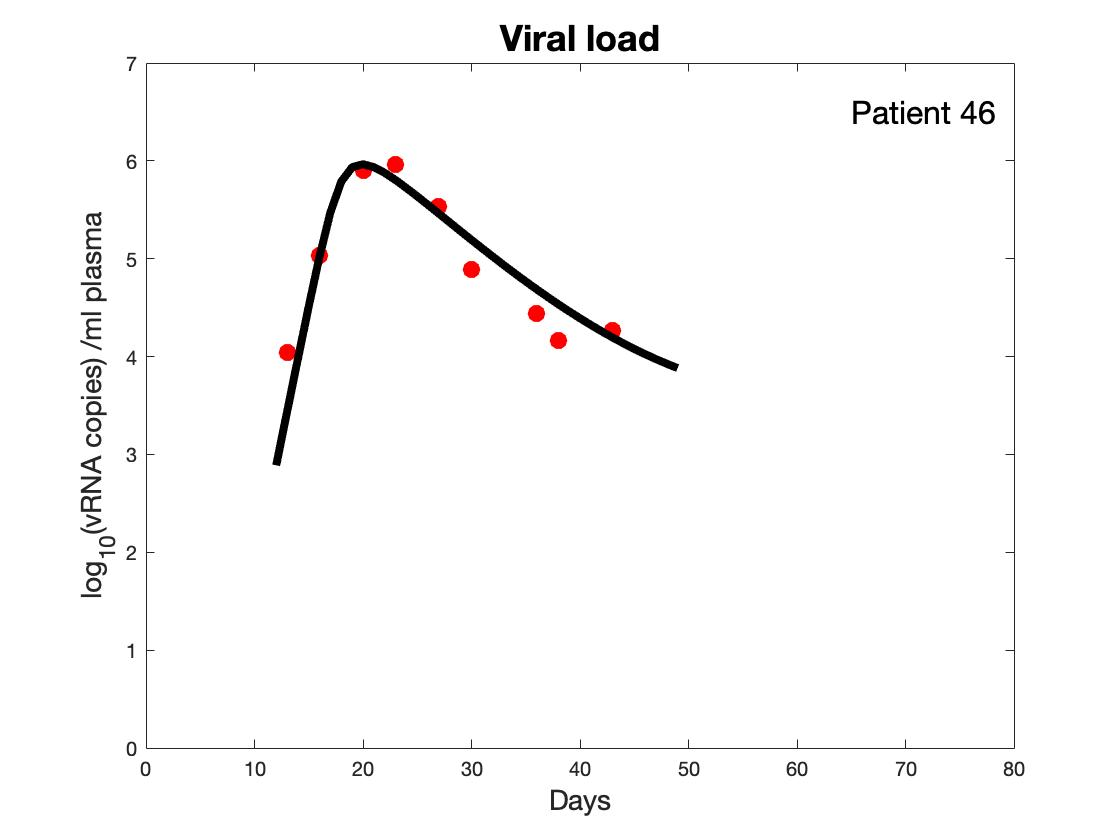
\includegraphics[width=.32\linewidth]{data_fit_app2/46v.jpg}
		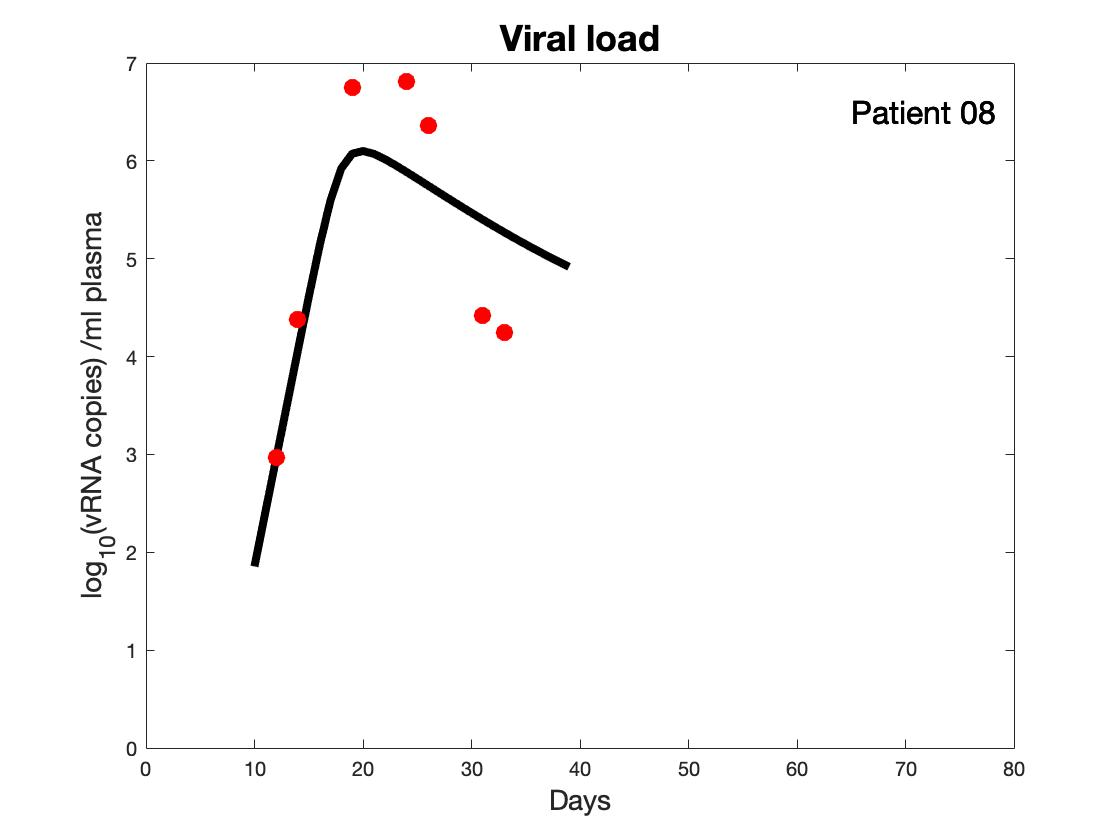
\includegraphics[width=.32\linewidth]{data_fit_app2/8v.jpg}
		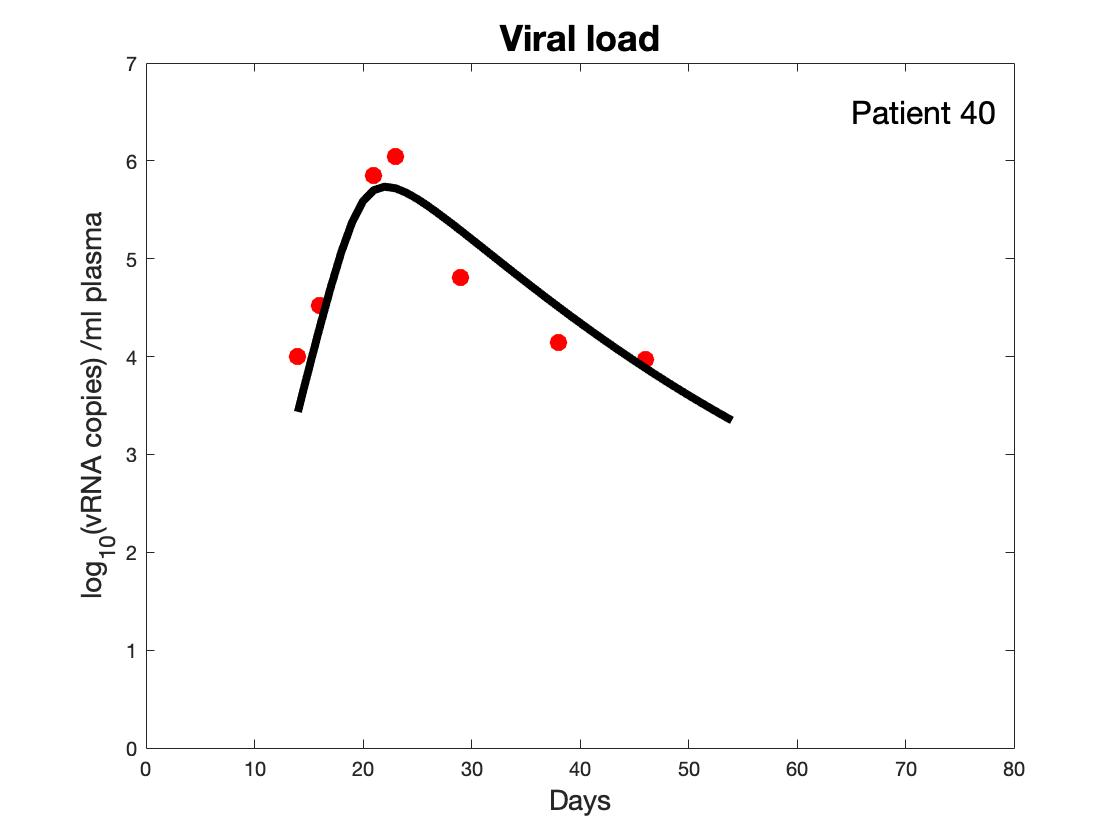
\includegraphics[width=.32\linewidth]{data_fit_app2/40v.jpg}
		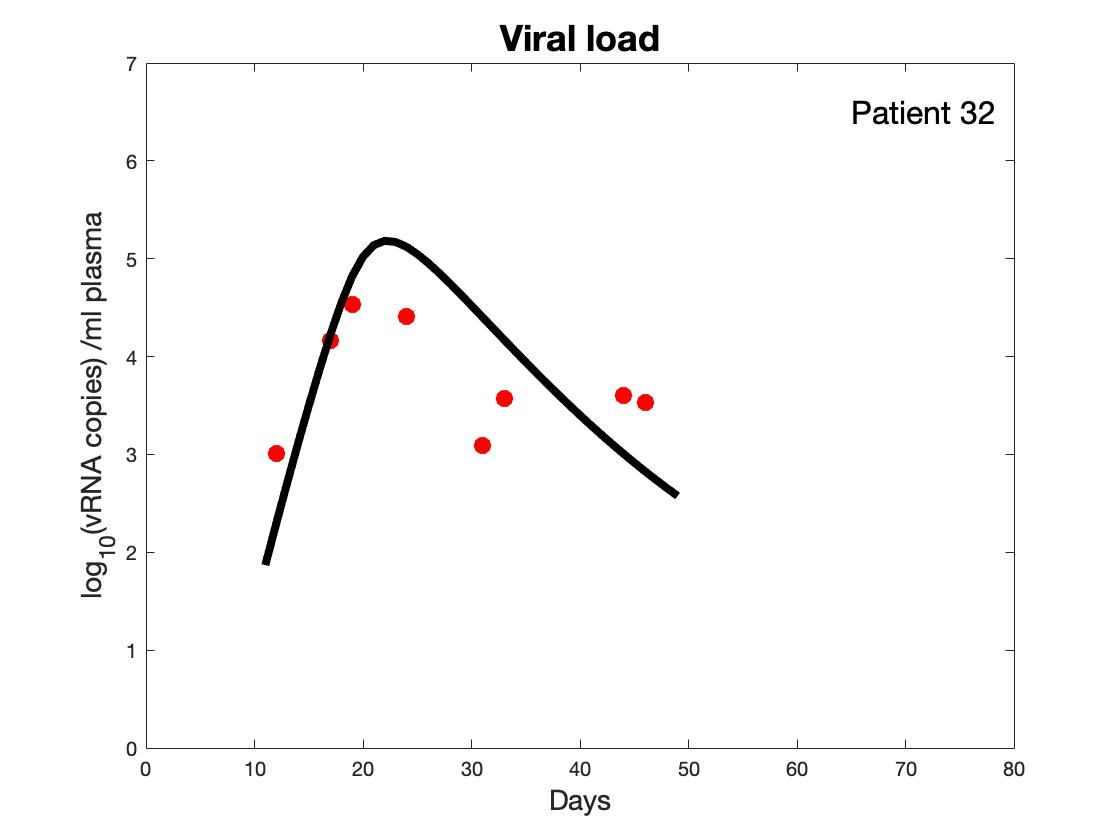
\includegraphics[width=.32\linewidth]{data_fit_app2/32v.jpg}
		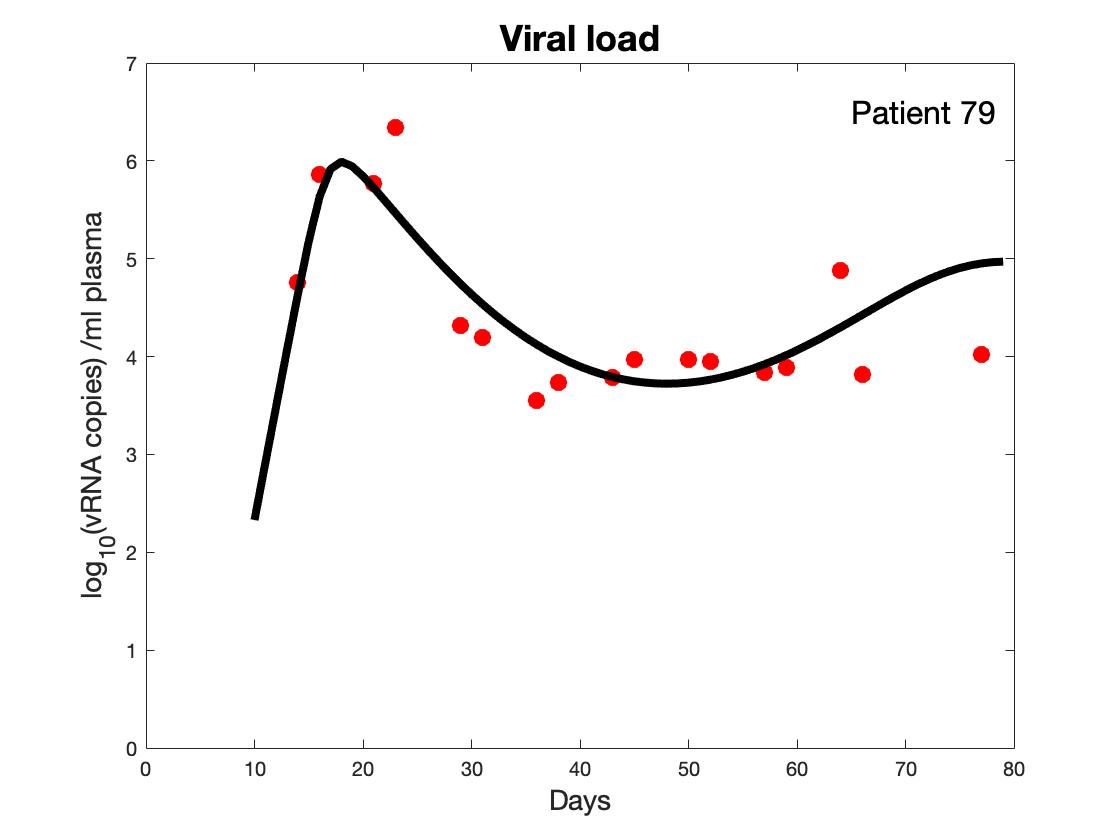
\includegraphics[width=.32\linewidth]{data_fit_app2/79v.jpg}
	\caption{Approach 2 viral load curve fitting}
	\label{app2viral}
\end{figure}



\begin{center}
\begin{table}[H]
\scriptsize
\centering
\begin{tabular}{c c c c c}
Parameter & Meaning & Value& Units\\ \hline
\textbf{Both approaches} \\ \hline
$\lambda$ & target cell production rate & $dT_0$& cell ml$^{-1}$ day$^{-1}$  \\
$p$ & production rate of Virus & 5000&virion day$^{-1}$ cell$^{-1}$ \\
$c$ & per capita clearance of virus& 23& 	day$^{-1}$\\
$d$ & per capita death rate of uninfected cells & $0.02, \hspace{1mm} 0.01$ &  day$^{-1}$\\
$k$ & mass Action infection rate & $7.39 \cdot 10^{-7}, \hspace{1mm}8.47\cdot 10^{-7}$  & ml day$^{-1}$ virion$^{-1}$\\
$\delta$ & 	per capita death rate of infected cells & $0.24, \hspace{1mm }0.28$ & day$^{-1}$ \\


\textbf{Approach 1}\\ \hline
$a$ & maximum antibody load& 2.5& O.D\\
$b$ & time at which $A(t) = M/2$& 40& day \\
$n$ & Hill's coefficient & 20.96 & O.D. day$^{-1}$ \\
$\varepsilon_A$ & efficacy of antibodies & dimensionless\\
$\mu$ & rate of viral clearance & 4.76 & O.D.$^{-1}$ day$^{-1}$\\
$\eta$& scaling factor in $\varepsilon_A$& 0.4& dimensionless \\

\textbf{Approach 2}\\ \hline

$\sigma$ & clearance rate of virus by antibodies& 13.092& O.D.$^{-1}$ day$^{-1}$\\
$\alpha$ & probability of virus being infectious & 0.9& dimensionless \\
$\ell$&Production rate of antibodies& $4.72\cdot10^{-7}$& ml O.D day$^{-1}$ virion$^{-1}$ \\
$w$ & death rate of antibodies& $4.15\cdot10^{-3}$& $day^{-1}$\\
\end{tabular}
\caption{Parameters for Model 1 \& 2 (lines with two values are listed as approach 1 estimate, approach 2 estimate }
\label{table:ta}
\end{table}
\end{center}



\subsection{Estimates of Risk of Infection}
Once we estimated all of our parameters, we took the median value of each parameter and used those values to calculate the probability of infection, c.f. Figure \ref{Pinfplot}. As previously stated, Wawer et al. \cite{Uganda} found the rate of HIV transmission per coital act was highest ($1/120 \approx 0.0083$) during the acute stage of infection and lowest ($1/670 \approx 0.001$) during the chronic stage of infection. In order to match our probability as much as possible to these results we had to take the $m$ value i.e. the proportion of the donor's viral load that is transmitted to the recipient to be $m = 0.00035$ for both approaches.
As can bee seen on the graph, the probability of transmission rises to a high of $\approx 0.1$ after 19-21 days post-infection during the acute stage before leveling off to $\approx$ 0.001 during the chronic stage. This probability of infection remains virtually unchanged throughout the chronic stage until the infection develops into AIDS (not pictured). We attribute the initial spike in the probability of infection to the high viral load and weak antibody response during the first month post-infection. It is important to take into account the age of the donor's infection, because as seen here the probability can be significantly higher depending on the stage of infection.

It is important to note that when antibodies are not included $\sigma = 0, \eta = 0, \mu = 0$, there is a significant difference in probabilities of transmission. In approach 2, we see the probability without antibodies is $1.7$ times higher, raising the peak probability from $0.07$ to $0.12$ (respectively $0.1$ to $0.084$ in approach 1). Furthermore, antibodies decrease the probability of transmission by roughly $86\%$ during the chronic stage.

\begin{figure}[H]
	\centering
		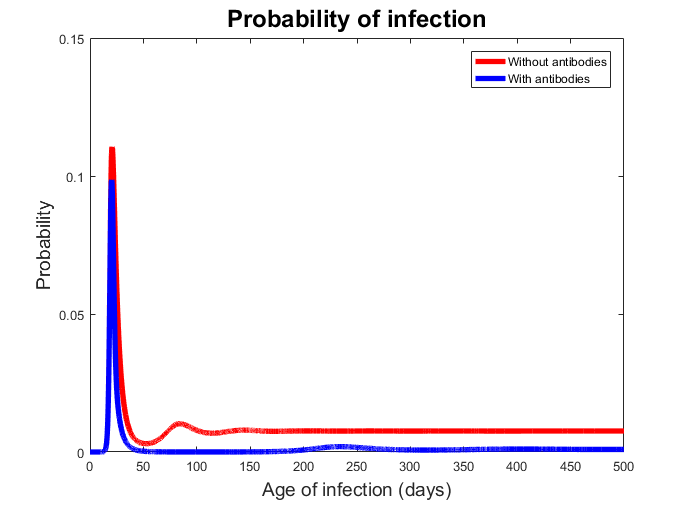
\includegraphics[width=.49\linewidth]{medianpinf.png}
		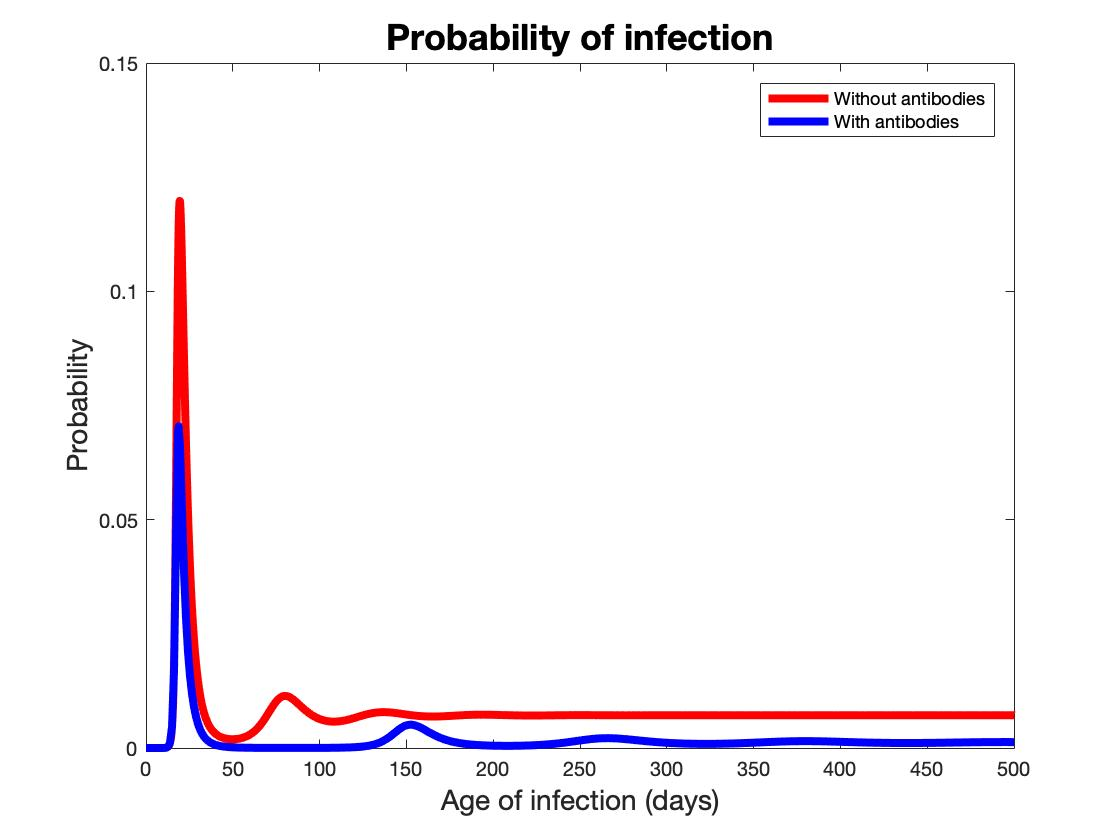
\includegraphics[width=.5\linewidth]{pinf2.jpg}
    \caption{Risk of infection for approach 1 (left) and approach 2 (right)}
	\label{Pinfplot}
\end{figure}

\subsection{Role of the Donor's Immune Status in the Risk of Infection}

The results of both approach 1 and 2 demonstrated in Figure \ref{Pinfplot} clearly show a correlation between the rise of antibodies in the donor and a decrease in the probability of HIV transmission. However, it should be strongly noted that even without antibodies, the probability of HIV transmission increases sharply the first few weeks after infection and then rapidly declines until it reaches a quasi-steady state that lasts until AIDS. Our results show how HIV-specific antibodies slightly to moderately reduce the peak probability of infection during the chronic stage, but play a larger role in reducing HIV transmission during the chronic stage when the probability of infection is already low. As a result, we believe that a decrease in probability of infection over time is an intrinsic property to HIV mostly due to a sharp decrease in virus concentration, with antibodies only playing a complementary role.

\subsection{Effect of the Route of Viral Entry}

As was previously noted, we assume some small proportion of the HIV and antibodies in the viral donor's bloodstream actually survives the transmission process. The proportion of the donor's viruses and antibodies that are released is represented by the scaling factor $m_1$ and the proportion of the released virus that enters the viral recipients blood stream is represented by the factor $m_2$. Consequently, the proportion of the donor's viral load that is transferred to the recipient is determined by that rate $m \in [0, 1]$ where $m=m_1m_2.$

The varying values of $m$ represent differing modes of viral transmission. A lower value for $m$ represents transmission types with a lower probability of infection, such as sexual transmission. In the case of sexual transmission, $m_1$ is the proportion of the donor's viral load and antibody count that is in the donor's semen. The value of $m_1$ is found by taking the product of the proportion of HIV-infected $CD4+T$ cells per milliliter of seminal fluid, and the average volume of seminal fluid from male ejaculation. A study on cell associated HIV mucousal transmission,  \cite{anderson2010} \cite{Xu1997}, found that the median HIV-infected population of $CD4+T$ cells in seminal fluid to be 0.2\% of the total white blood cell count in seminal fluid. From a review of 30 articles, \cite{Xu1997} concludes that the average volume of seminal fluid is 3.4ml. So the proportion of infectious $CD4+T$ cells that are released by an HIV-infected male is $m_1$ = 0.0068.

$m_2$ is proportion of the viruses and antibodies in the viral donor's semen that permeates the mucus membranes of the recipient and thus enters the recipients blood stream. While there has not been a quantification of the natural resistance of the vaginal mucus membrane to HIV-infected $CD4+T$ cells, \cite{Wira2015}\cite{Cutler2008}\cite{Tebit2012}, suggest that a variety of natural defenses are in place to prevent HIV infection through vaginal intercourse. Primarily, these defenses come from the secretion of glycoproteins, cytokines, chemokines and antimicrobial proteins by the endocervical epithelial cells. In line with prevailing knowledge on the probability of HIV infection through vaginal intercourse, we estimate that the natural immune defenses of the mucus membrane in the vaginal tract to reduce the proportion of infectious $CD4+T$ cells by a factor of $m_2 = \frac{1}{25}$. Consequently $m$ = $m_1 m_2$ = 0.0003.



A higher value for $m$ represents more direct transmission types, transmission types with a higher probability of infection for the viral recipient. Thus, a higher $m$ value is associated with transmission types such as needle sticks in injection drug use and blood transfusions.
For the case of transmission via needle stick, $m_1$ is the portion of the viral donor's blood that remains on the needle and $m_2$ is the portion of the infected blood on the needle that is transferred to the recipient. Due to the nature of this transmission type, the value of $m_2$ is much higher compared to the value of $m_2$ from sexual transmission.

An inspection of the effect of varying values of $m$ on the probability of infection shows that the transmission type has a significant effect on the probability that the viral recipient becomes infected, which in turn has a significant effect on the outcome of the model. Figure \ref{sens} shows at one month and one year respectively the affect of transmission type on the probability of infection increases. Furthermore, since the value of $m$ is scaled in part by the natural defense mechanisms of the vaginal mucus membrane, Figure \ref{sens} also demonstrates the importance of accurately quantifying the effectiveness of the vaginal mucus membranes ability in preventing an infection \cite{Owen2005}.

\begin{figure}[H]
    \centering
        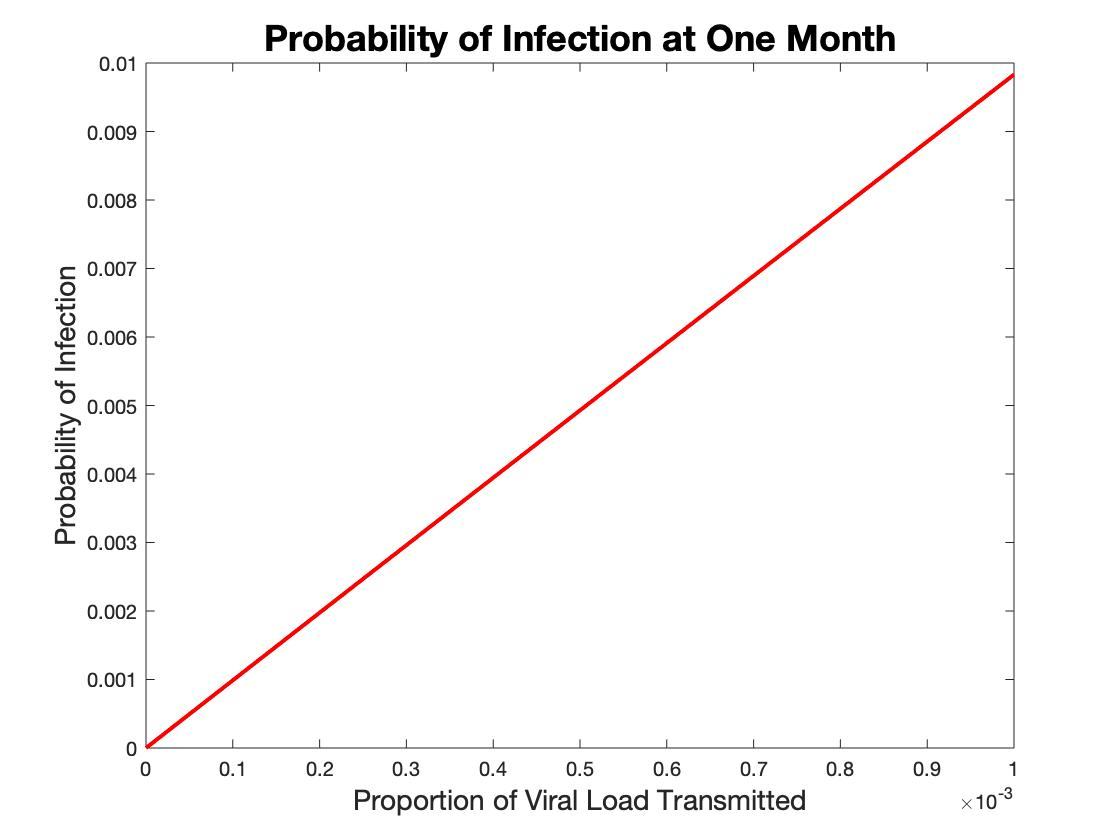
\includegraphics[width=.49\linewidth]{MSENS2.jpg}
        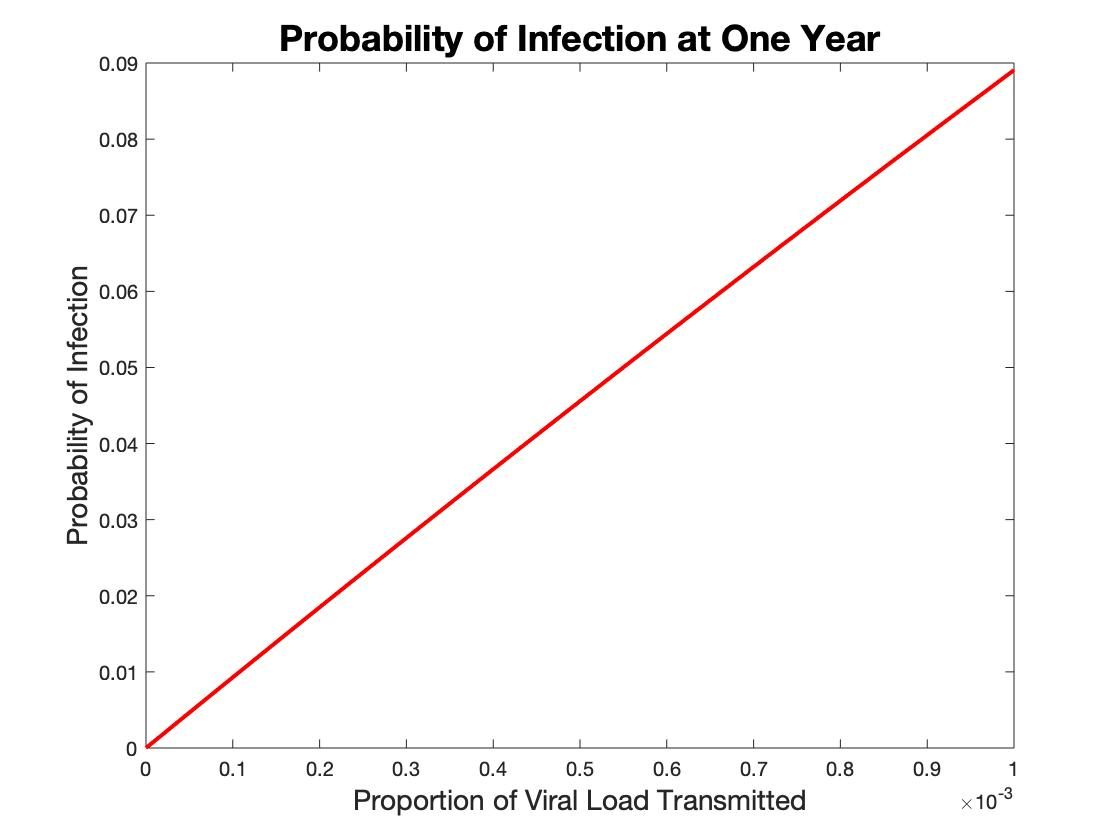
\includegraphics[width=.49\linewidth]{MSENS4.jpg}
    \caption{Sensitivity analysis on $m$'s effects on probability}
    \label{sens}
\end{figure}

\section{Discussion}
The standard HIV model \cite{perelson2013modeling} treats HIV using a three-compartment model, considering the interactions of viruses with infected and uninfected CD4$^+$T cells, but does not consider the effects of antibodies. While developing a theory of the risk of infection, we extended this model to incorporate the effects of antibodies, in order to show that the inclusion of antibody dynamics and the effects of antibodies on free-floating viruses increases the accuracy of HIV modeling. As depicted in Figure \ref{Pinfplot}, this adaption presented a significant change in the viral dynamics of the system, reducing the probability of infection.

We considered two different approaches to introduce antibodies into the model. By basing our representation of antibodies from both an external empirical source, as in approach 1, and from the dynamical system, as in approach 2, we are able to compare the two models for accuracy. Since two models with different assumptions, both included antibodies, agreed qualitatively on the effect of antibodies on the probability of transmission, we believe that the results of our model to be credible.

In approach 1, we treated antibody profile as a function that is not directly influenced by the viral dynamics of our model, and fit the function to available patient data \cite{CHIDPatients}. Subsequently, we used the function for antibodies to scale the rate at which viruses infected susceptible CD4$^+$T cells and active viruses become neutralized. While approach 1 does not directly demonstrate the dynamics between the antibody profile and viral load of an infected host, approach 1 does demonstrate the effect that antibodies have upon the viral dynamics on an infected individual as a whole. However, our ability to fit the antibody function was limited by the size of the patient antibody data that was available; we had access to the data of only six patients. In approach 2, we represented antibodies and noninfectious viruses separate compartments in the model, so that the behavior of antibodies is directly affected by the viral dynamics of the model. approach 2 thus demonstrates the direct relation to the interplay between the level of antibodies and infectious viruses in an infected individual. Since Approach 2 does not model antibody profile as a function and therefore has more parameters, it is more difficult to fit to data, but is easier to do theoretical work with since it is a constant-coefficient system.

The transmission proportion is a new parameter which describes the proportion of viruses, infected CD4$^+$T cells, and antibodies that are transferred between the viral host and susceptible viral recipient per sexual contact. We factor $m$ as $m = m_1m_2$, where $m_1$ is the proportion of viruses, infected CD4$^+$T cells, and antibodies in the seminal discharge of the infected individual, and $m_2$ is the proportion of viruses, infected CD4$^+$T cells, and antibodies that travel through the vaginal mucus membrane of the viral recipient. The value of $m$ has a significant effect upon the probability of infection per sexual contact; therefore, future work should aim to find a more precise, empirically supported value of $m$. Moreover, in future work, it would be prudent to add a third factor, $m_3$, to represent of effects of antiretroviral therapy. As with $m_1$ and $m_2$, the value of $m_3$ would be a scaling value for the reduction in the proportion of the viral donor's viral load that infects a viral recipient. The introduction of antiretroviral therapy as the value $m_3$ would have a similar effect as the values of $m_1$ and $m_2$ on the reduction in the probability of viral infection between a viral donor and viral recipient.

Previous studies have treated the risk of infection either as constant or as constant within each of the acute and chronic stages; we can now consider the risk of infection as a continuous function of time. In the first two weeks into infection, which we call eclipse stage, a newly infected donor with low viral load and no antibodies has almost zero infection risk. In other words, our findings suggest that in the days immediately after infection, the viral load is simply not high enough to be transmitted, even though antibodies have not yet formed. On the other hand, in the following weeks, up to approximately the end of the second month, the risk of transmission is extremely high, spiking at around $1$ transmission per $10$ sexual acts, and sexual contact becomes extremely risky. As the system stabilizes, the effects of antibodies dominate and the probability of infection levels off (and is much higher if we ignore the effects of antibodies). In a future paper, we will apply our computation of the risk of infection to a between-host model which treats the number of infected individuals of a given age of infection using an age-structure equation, in order to better compute the prevalence, death count, and other statistics of a hypothetical HIV outbreak.
\phantom{\cite{Stafford2000}
\cite{Vaidya2010}
\cite{Song2007}
\cite{VaidyaTreatment}
\cite{Cai2009}
\cite{Rahman2014}
\cite{Nargesalsadat2017}}

\section*{References}
\bibliography{references}


\cleardoublepage


%%%%%%%%%%%%%%%%%%%%%%%%%%%%%%%%%%%%%%%%%%%%%%%%%%%%%%%%%%%%%%%%%%%%%%%%%%%%%%%%%%%%%%%%%%%%%%%%%%%%%%%%%%%%%%%%%%%%%%%%%%%%%%%%%%%%%%%%%%%%%%%%%%%%%%%%%%%%%%%%%%

\begin{appendices}
\section{Proof of Theorem \ref{ife_theorem}: viral extinction and asymptotic stability}


%%%%%%%%%%%%%%%%%%%%%%%%%%%%%%%%%%%%%
%%%%%%%%%%%%%%%%%%%%%%%%%%%%%%%%%%%%%%%%%%%%%%%%%%%%%%%%%%%%%%%%%%%%%%%%%%

Different proofs are required for each Approach.

\subsection{Approach 1}
\label{global1}
Let $\beth \in (0, 1)$ be arbitrary. Since $A \to M$ as $t \to \infty$, we can choose $t_0 > 0$ so large that if $t \geq t_0$, then $\varepsilon_A > 1 - \beth$ and $A > M - \beth$. Therefore there are $\tilde k < k$ and $\tilde c > c$ such that whenever $t > t_0$, one has
\begin{align*}
    \lambda - dT - kTV &\leq \dot T \leq \lambda - dT - \tilde kTV\\
    \tilde kTV - \delta I &\leq \dot I \leq kTV - \delta I\\
    pI - \tilde cV &\leq \dot V \leq pI - cV.
\end{align*}
    Denote the Jacobian of the classical model
\begin{align*}
    \dot T &= \lambda - dT - kTV\\
    \dot I &= kTV - \delta I\\
    \dot V &= pI - cV,
\end{align*}
    linearized about $\IFE$ by
    $$J = \begin{bmatrix}-d&k \lambda/d&0\\0&-\delta&0\\0&p&-c\end{bmatrix}.$$
    Clearly $J$ is negative definite, and it remains such as $k$ and $c$ are allowed to vary to $\tilde k$ and $\tilde c$ provided that $\beth$ is small enough. Therefore in a neighborhood of this strip, the classical model has no bifurcations, so that it depends on continuously on the parameters. So solution curves of the Approach 1 model are sandwiched between solutions of the classical model with parameters $k,c$ and the classical model with approximate parameters $\tilde k, \tilde c$. Moreover, the $\BRN$s of the classical model with approximate parameters and classical model are both bounded above by the $\BRN$ of Approach I, which is $< 1$.

    The classical model and the classical model with approximate parameters can both be easily shown to be globally asymptotically stable at $\IFE$ whenever $\BRN < 1$; the proof is the same as Theorem 3.2 of \cite{rahman2016impact}. Since the solution curves are sandwiched, the Approach 1 model is globally asympotically stable as well.
%%%%%%%%%%%%%%%%%%%%%%%%%%%%%%%%%%%%%%%%%%%%%%%%%%%%%%%%%%%%%%%%%%%%%%%%%%%%%%%%%%%%%%%%%%%%%%%%%%%%%%%%%%%%%%%%%%%%%%%%%%%%%%%%%%%%%%%%%%%%%%%%%%%%%%%%%%%%%%%%%%
\subsection{Approach 2}
\label{global2}
 The argument for Approach 2 was based on an argument in \cite{Lyapunov}.

\label{app1b}
By definition,
$$kT_0 = \frac{c \delta}{\alpha p} \BRN.$$Consider the smooth function
$$L(T, I, V_I, V_N, A) = T - T_0\left(1 + \ln\frac{T}{T_0}\right) + I + \frac{\delta}{\alpha p} V_I.$$
Then $L(\IFE) = 0$ and $$\nabla L = \left(1 - \frac{T_0}{T}, 1, \frac{\delta}{\alpha p}, 0, 0\right)$$
whence the only critical points are the line $T = T_0$ (on which $L \leq 0$), and
$\lim_{T \to 0} L = +\infty$
it follows that $L \leq 0$. Moreover,
\begin{align*}
    \dot L &= \left(1 - \frac{T_0}{T} \right)(\lambda - dT - kTV_I) + kTV_I - \delta I + \frac{\delta}{\alpha p}(\alpha p I - cV_I - \sigma A V_I)\\
    &\leq kT_0 V_I + dT_0 - \lambda \frac{T_0}{T} - kTV_I - dT + \lambda + kTV_I - \delta I + \delta I - \frac{\delta c}{\alpha p} V_I\\
    &\leq d(T_0 - T) +kT_0 V_I -\frac{\delta c}{\alpha p} V_I
    \leq d\left(\frac{T_0}{T} - 1\right)(T - T_0) + \left(kT_0 - \frac{c\delta}{\alpha p}\right) V_I\\
    &= d\left(\frac{T_0}{T} - 1\right)(T - T_0) + V_I \frac{c \delta}{\alpha p}(\BRN - 1) \leq 0
\end{align*}

with equality iff $T = T_0$ and $V_I = 0$. Thus, $L$ is strictly Lyapunov on $\BB$. So by Lyapunov's theorem (proven in, e.g., \cite{robert2004differential}), $\IFE$ is asymptotically stable on $\BB$.

Now we shall consider a solution curve $Z$ satisfying the initial conditions $T(0) = T_0$ and $V_I(0) = 0$. If $I(0) = 0$ also then it is easy to see that $(V_N, A) \to (0, 0)$, whence $X \to \IFE$. We therefore now must treat the edge case that the body is infected but $V_I(0) = 0$. Then $I(0) > 0$, so $\dot{V_I}(0) = pI(0) > 0$. Thus there is a $\varepsilon > 0$ such that $V_I(\varepsilon) > 0$. Translating back in time by $\varepsilon$ we arrive at a solution curve $\tilde Z$ for which $V_I(0) > 0$, whence $\tilde Z$ tends to $\IFE$. Thus $Z \to \IFE$ also. This completes the proof.
%%%%%%%%%%%%%%%%%%%%%%%%%%%%%%%%%%%%%%%%%%%%%%%%%%%%%%%%%%%%%%%%%%%%%%%%%%%%%%%%%%%%%%%%%%%%%%%%

\section{Proof of Theorem \ref{IE}: uniform persistence}

\label{pers}
    If we are in the situation of Approach I, let $\alpha = 1$ in what follows. Otherwise the proofs for the two Approaches are identical.

    Let $\mathcal W$ denote the stable manifold of $\IFE$. At $\IFE$, the Jacobian $J = F - V$ has determinant $\det J = c\delta - kp\alpha\lambda d^{-1}$. Assuming that $\BRN > 1$, $\det J \neq 0$. Therefore $\IFE$ is hyperbolic, so by the stable manifold theorem (proven in, e.g., \cite{dyatlov2018notes}), it suffices to show that $\mathcal W \cap \BB$ is empty.

    Suppose that $(T, X, V_N, A) \in \mathcal W \cap \BB$. Let
    $$\tilde T(\varepsilon) = \frac{T_0 - \varepsilon}{T_0 + \varepsilon} < 1$$ and let $D = \tilde TF - V$, so that $\dot X = JX \geq D(\varepsilon)X$, the inequality taken pointwise. If $\sigma(\varepsilon)$ is the spectrum of $D(\varepsilon)$, then Theorem 2 of \cite{van2002reproduction} implies that $\sigma(0) = \operatorname{Spec} J$ has a positive element. Clearly $\sigma$ is continuous, so if $\varepsilon$ is small enough, $D(\varepsilon)$ has a positive element $\lambda$. Therefore there is a basis and an index $j \in \{1, 2\}$ such that we can write $X = (X_1, X_2)$ and such that $\dot X_j \geq \lambda X_j > 0$, so $X$ blows up. But $X \in \mathcal W$ so this is a contradiction.



With a persistent infection, we can conclude that there is a positive equilibrium of the system. If we are allowed to assume that $T$, $I$, $V_I$, $V_N$, and $A$ for approach 2 are all very large, then we are justified in using the deterministic ODE models previously given. In this case, we let $IE = (T^*, I^*, V_I^*, V_N^*, A^*)$ be the infectious equilibrium. Assuming that $T = T^*$, $I = I^*$, $V_I = V_I^*$, $V_N = V_N^*$, and $A = A^*$, we have $\dot T = \dot I = \dot V_I = \dot V_N = \dot A = 0$, so the model reduces to a system of algebraic equations. For Approach 2, a symbolic approach in MATLAB then gives
\begin{align*}
    T^* &= \frac{w\delta c^2+\ell\lambda p\sigma}{p(\ell d\sigma+\alpha wck)},\\
    I^* &= \frac{wc^2 d}{\delta} \frac{\BRN - 1}{\ell d\sigma + \alpha wck},\\
    V_I^* &= wc^2d\delta\frac{\BRN - 1}{w\delta kc^2 + \ell k\lambda p\sigma},\\
    A^* &= \ell cd \frac{\BRN - 1}{\ell d \sigma + \alpha wck},\\
    V_N^* &= \frac{w}{\ell}A^* - V_I^*.
\end{align*}

%%%%%%%%%%%%%%%%%%%%%%%%%%%%%%%%%%%%%%%%%%%%%%%%%%%%%%%%%%%%%%%%%%%%%%%%%%%%%%%%%%%%%%%%%%%%%%%%%%%%%%%%%%%%%%%%%%%%%%%%%%%%%%%%%%%%%%%%%%%%%%%%%%%%%%%%%%%%%%%%%%%%%%%%%%%%%%%



\end{appendices}

\end{document}
